\subsection{Caso d'uso \hyperref{UC1}{UC1}: Registrazione }
\begin{figure} [H]
\centering
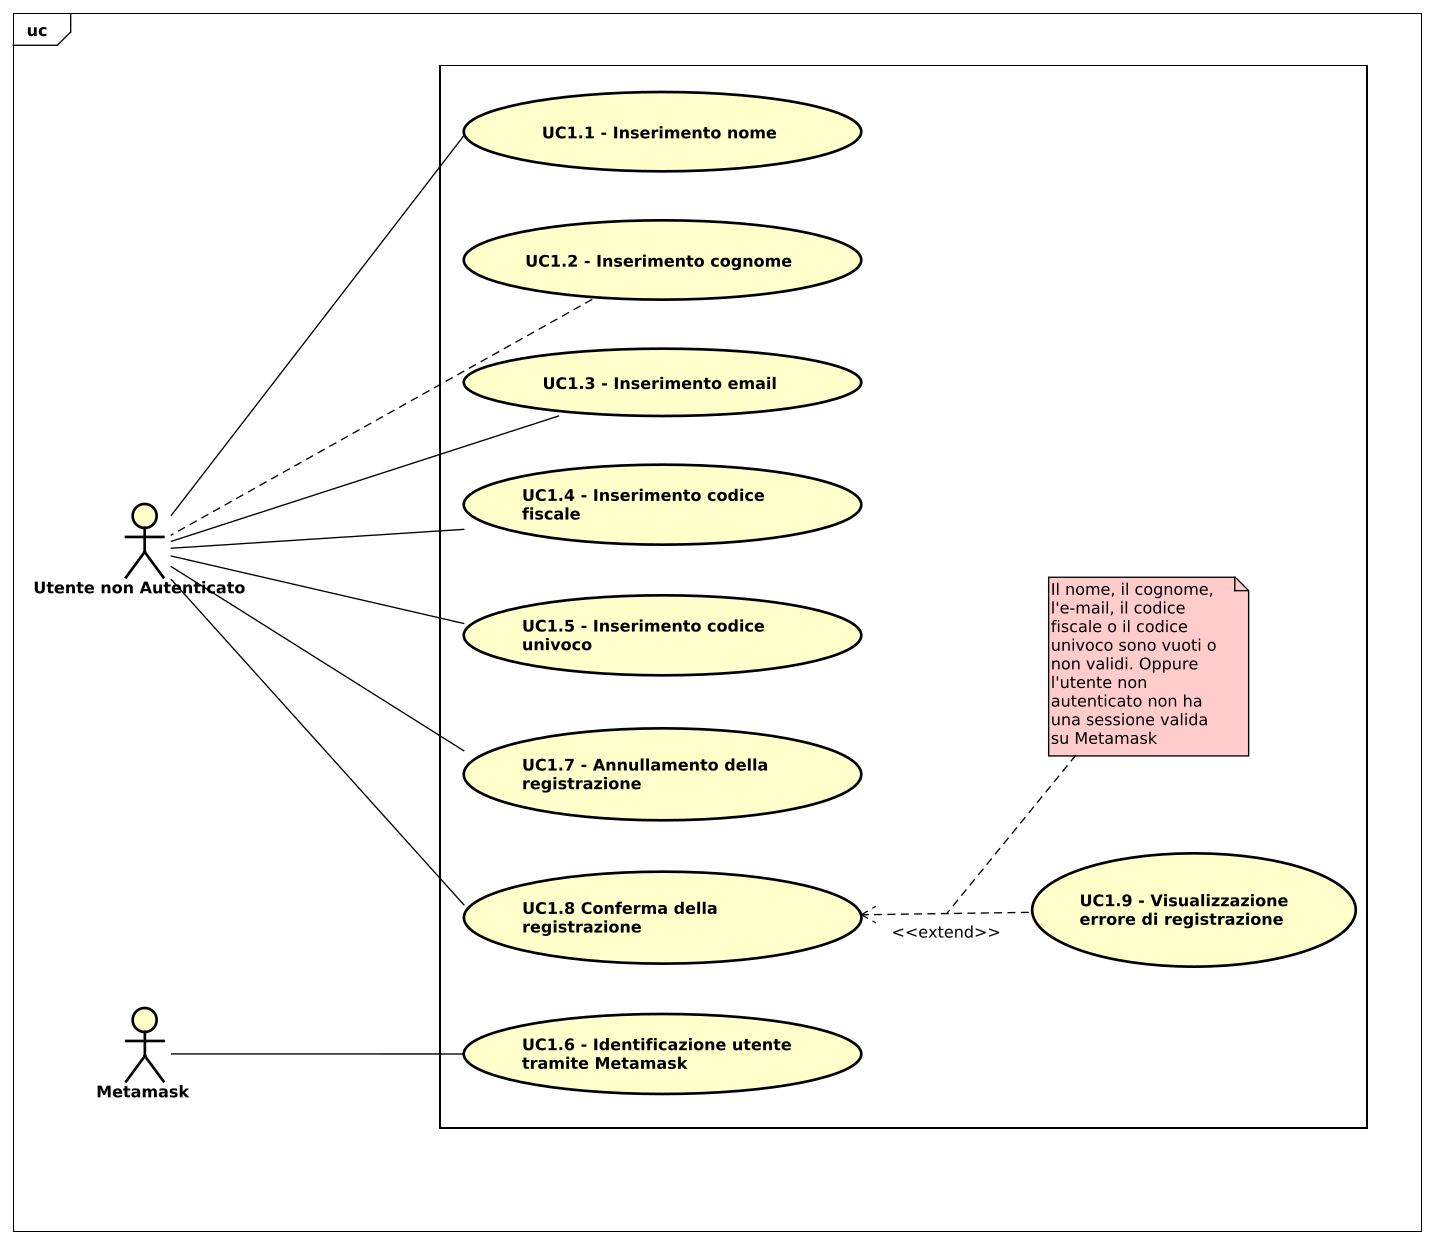
\includegraphics[scale=0.45]{./img/UC1.png}
\caption{Registrazione }\label{}
\end{figure}
\begin{itemize}
\item \textbf{Attori}: Metamask, utenteNonAutenticato
\item \textbf{Descrizione}: Per accedere al sistema è necessario possedere un account.
\item \textbf{Precondizione}: L'attore non possiede una account per accedere al sistema.
\item \textbf{Flusso principale degli eventi}: L'attore vuole registrarsi nel sistema;
\begin{itemize}
\item Inserimento nome (UC1.1)
\item Inserimento cognome (UC1.2)
\item Inserimento e-mail (UC1.3)
\item Inserimento codice fiscale (UC1.4)
\item Inserimento codice univoco (UC1.5)
\item Il sistema sfrutta l'interfaccia Metamask per l'identificazione utente (UC1.6)
\item Annullamento della registrazione (UC1.7)
\item Conferma della registrazione (UC1.8)
\item Visualizzazione errore di registrazione (UC1.9)
\item Inserimento matricola (UC1.10)
\end{itemize}
\item \textbf{Postcondizione}: L'attore ha creato un account per accedere al sistema.
\end{itemize}
\subsection{Caso d'uso \texorpdfstring{UC1.1}{UC1.1}: Inserimento nome}
\begin{itemize}
\item \textbf{Attori}: utenteNonAutenticato
\item \textbf{Descrizione}: L'attore deve inserire il proprio nome per potersi registrare.
\item \textbf{Precondizione}: L'attore visualizza il campo di inserimento del nome.
\item \textbf{Flusso principale degli eventi}: L'attore inserisce il proprio nome per effettuare la registrazione.
\item \textbf{Postcondizione}: L'attore ha inserito il nome.
\end{itemize}
\subsection{Caso d'uso \texorpdfstring{UC1.2}{UC1.2}: Inserimento cognome}
\begin{itemize}
\item \textbf{Attori}: utenteNonAutenticato
\item \textbf{Descrizione}: L'attore deve inserire il proprio cognome per potersi registrare.
\item \textbf{Precondizione}: L'attore visualizza il campo di inserimento del cognome.
\item \textbf{Flusso principale degli eventi}: L'attore deve inserire il cognome per potersi registrare.
\item \textbf{Postcondizione}: L'attore ha inserito il cognome.
\end{itemize}
\subsection{Caso d'uso \texorpdfstring{UC1.3}{UC1.3}: Inserimento e-mail}
\begin{itemize}
\item \textbf{Attori}: utenteNonAutenticato
\item \textbf{Descrizione}: L'attore deve inserire la proprio e-mail per potersi registrare.
\item \textbf{Precondizione}: L'attore visualizza il campo di inserimento dell'e-mail.
\item \textbf{Flusso principale degli eventi}: L'attore inserisce la propria e-mail per effettuare la registrazione.
\item \textbf{Postcondizione}: L'attore ha inserito la propria e-mail.
\end{itemize}
\subsection{Caso d'uso \texorpdfstring{UC1.4}{UC1.4}: Inserimento codice fiscale}
\begin{itemize}
\item \textbf{Attori}: utenteNonAutenticato
\item \textbf{Descrizione}: L'attore deve inserire il proprio codice fiscale per potersi registrare.
\item \textbf{Precondizione}: L'attore visualizza il campo di inserimento del codice fiscale.
\item \textbf{Flusso principale degli eventi}: L'attore inserisce il proprio codice fiscale per effettuare la registrazione.
\item \textbf{Postcondizione}: L'attore ha inserito il codice fiscale.
\end{itemize}
\subsection{Caso d'uso \texorpdfstring{UC1.5}{UC1.5}: Inserimento codice univoco}
\begin{itemize}
\item \textbf{Attori}: utenteNonAutenticato
\item \textbf{Descrizione}: L'attore inserisce il codice univoco rilasciato dall'università per la registrazione.
\item \textbf{Precondizione}: L'attore visualizza il campo di inserimento del codice univoco.
\item \textbf{Flusso principale degli eventi}: L'attore inserisce il codice univoco per effettuare la registrazione.
\item \textbf{Postcondizione}: L'attore ha inserito il codice univoco.
\end{itemize}
\subsection{Caso d'uso \texorpdfstring{UC1.6}{UC1.6}: Il sistema sfrutta l'interfaccia Metamask per l'identificazione utente}
\begin{itemize}
\item \textbf{Attori}: Metamask
\item \textbf{Descrizione}: Il sistema sfrutta l'interfaccia Metamask per poter identificare univocamente l'utente;
\item \textbf{Precondizione}: Il sistema è fermo sulla pagina di registrazione utente;
\item \textbf{Flusso principale degli eventi}: Il sistema ha bisogno dell'interfaccia Metamask per poter registrare un utente.
\item \textbf{Postcondizione}: Il sistema ha identificato l'utente.
\end{itemize}
\subsection{Caso d'uso \texorpdfstring{UC1.7}{UC1.7}: Annullamento della registrazione}
\begin{itemize}
\item \textbf{Attori}: utenteNonAutenticato
\item \textbf{Descrizione}: L'attore decide di annullare la registrazione in corso;
\item \textbf{Precondizione}: L'attore sta effettuando la registrazione nel sistema;
\item \textbf{Flusso principale degli eventi}: L'attore decide di annullare la registrazione in corso.
\item \textbf{Postcondizione}: L'attore ha annullato la registrazione nel sistema;
\end{itemize}
\subsection{Caso d'uso \texorpdfstring{UC1.8}{UC1.8}: Conferma della registrazione}
\begin{itemize}
\item \textbf{Attori}: utenteNonAutenticato
\item \textbf{Descrizione}: L'attore può aver inserito tutti i dati  e conferma la registrazione;
\item \textbf{Precondizione}: L'attore può confermare la registrazione;
\item \textbf{Flusso principale degli eventi}: L'attore dopo aver inserito i dati può completare la registrazione confermandola.
\item \textbf{Postcondizione}: L'attore ha confermato la registrazione;
\item \textbf{Estensioni}:
\begin{itemize}
\item Visualizzazione errore di registrazione (UC1.9)
\end{itemize}
\end{itemize}
\subsection{Caso d'uso \texorpdfstring{UC1.9}{UC1.9}: Visualizzazione errore di registrazione}
\begin{itemize}
\item \textbf{Attori}: utenteNonAutenticato
\item \textbf{Descrizione}: L'attore può visualizzare un errore nel caso avesse inserito dati errati;
\item \textbf{Precondizione}: Il sistema ha ricevuto campi dati errati o vuoti;
\item \textbf{Flusso principale degli eventi}: L'attore visualizza un messaggio d'errore relativo all'inserimento mancato o non valido di:
\begin{itemize}
\item nome;
\item cognome;
\item e-mail;
\item codice fiscale;
\item codice univoco;
\item matricola;
\end{itemize}
\item \textbf{Postcondizione}: Il sistema visualizza un messaggio d'errore;
\end{itemize}
\subsection{Caso d'uso \texorpdfstring{UC1.10}{UC1.10}: Inserimento matricola}
\begin{itemize}
\item \textbf{Attori}: utenteNonAutenticato
\item \textbf{Descrizione}: L'attore inserisce la matricola ad esso associato dall'università per la registrazione
\item \textbf{Precondizione}: L'attore visualizza il campo di inserimento della matricola
\item \textbf{Flusso principale degli eventi}: L'attore inserisce la matricola per effettuare la registrazione
\item \textbf{Postcondizione}: L'attore ha inserito la matricola
\end{itemize}
\subsection{Caso d'uso \texorpdfstring{UC2}{UC2}: Login}
\begin{figure} [H]
\centering
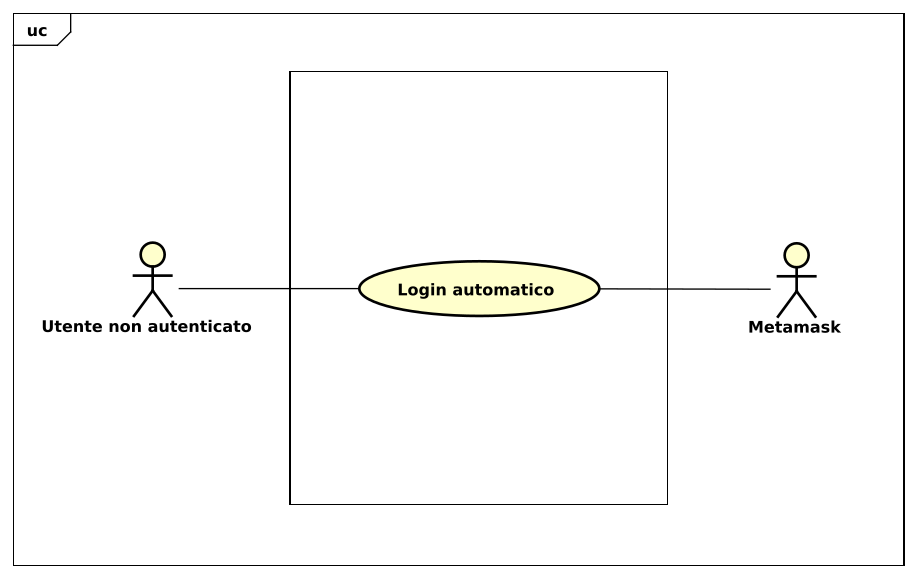
\includegraphics[scale=0.45]{./img/UC2.png}
\caption{Login}\label{}
\end{figure}
\begin{itemize}
\item \textbf{Attori}: utenteNonAutenticato
\item \textbf{Descrizione}: Il sistema è avviato ma è necessario loggarsi per accedervi.
\item \textbf{Precondizione}: L'attore non ha accesso al sistema.
\item \textbf{Flusso principale degli eventi}: L'attore effettua automaticamente il login;
\begin{itemize}
\item Login automatico (UC2.1)
\end{itemize}
\item \textbf{Postcondizione}: L'attore si è loggato e ha accesso al sistema.
\end{itemize}
\subsection{Caso d'uso \texorpdfstring{UC2.1}{UC2.1}: Login automatico}
\begin{itemize}
\item \textbf{Attori}: Metamask, utenteNonAutenticato
\item \textbf{Descrizione}: Il sistema logga automaticamente l'attore se ha metamask attivo e la sua chiave pubblica coincide con una presente all'interno del sistema;
!!Metamask attore secondario!!
\item \textbf{Precondizione}: L'attore entra nel sito e non è riconosciuto dal sistema;
\item \textbf{Flusso principale degli eventi}: L'attore con Metamask attivo e precedentemente registrato, entra nel sistema senza compiere alcuna azione;
\item \textbf{Postcondizione}: L'attore viene riconosciuto dal sistema;
\end{itemize}
\subsection{Caso d'uso \texorpdfstring{UC3}{UC3}: Aggiunta di un anno accademico}
\begin{figure} [H]
\centering
\includegraphics[scale=0.45]{./img/UC3.png}
\caption{Aggiunta di un anno accademico}\label{}
\end{figure}
\begin{itemize}
\item \textbf{Attori}: università;
\item \textbf{Descrizione}: L'attore aggiunge un anno accademico alla lista degli anni accademici;
\item \textbf{Precondizione}: La lista degli anni accademici è vuota oppure non contiene l'anno accademico che l'attore vuole inserire;
\item \textbf{Flusso principale degli eventi}: L'attore, per inserire l'anno accademico alla lista, deve seguire i seguenti punti:
\begin{itemize}
\item Inserimento dell'inizio dell'anno accademico (UC3.1)
\item Inserimento della fine dell'anno accademico (UC3.2)
\item Annullamento dell'aggiunta dell'anno accademico (UC3.3)
\item Conferma dell'aggiunta di un anno accademico (UC3.4)
\item Visualizzazione errore relativo all'aggiunta di un anno accademico non valido (UC3.5)
\item Aggiunta di un corso di laurea (UC3.6)
\item Modifica di un corso di laurea (UC3.7)
\item Eliminazione del corso di laurea (UC3.8)
\end{itemize}
\item \textbf{Postcondizione}: La lista degli anni accademici contiene l'anno accademico che l'attore voleva inserire;
\end{itemize}
\subsection{Caso d'uso \texorpdfstring{UC3.1}{UC3.1}: Inserimento dell'inizio dell'anno accademico}
\begin{itemize}
\item \textbf{Attori}: università;
\item \textbf{Descrizione}: L'attore compila il campo relativo all'inizio dell'anno accademico;
\item \textbf{Precondizione}: L'attore può impostare l'inizio dell'anno accademico;
\item \textbf{Flusso principale degli eventi}: L'attore imposta l'inizio dell'anno accademico;
\item \textbf{Postcondizione}: L'attore ha impostato l'inizio dell'anno accademico.
\end{itemize}
\subsection{Caso d'uso \texorpdfstring{UC3.2}{UC3.2}: Inserimento della fine dell'anno accademico}
\begin{itemize}
\item \textbf{Attori}: università;
\item \textbf{Descrizione}: L'attore compila il campo relativo alla fine dell'anno accademico;
\item \textbf{Precondizione}: L'attore può impostare la fine dell'anno accademico;
\item \textbf{Flusso principale degli eventi}: L'attore imposta la fine dell'anno accademico;
\item \textbf{Postcondizione}: L'attore ha impostato la fine dell'anno accademico.
\end{itemize}
\subsection{Caso d'uso \texorpdfstring{UC3.3}{UC3.3}: Annullamento dell'aggiunta dell'anno accademico}
\begin{itemize}
\item \textbf{Attori}: università;
\item \textbf{Descrizione}: L'attore può voler più aggiungere un anno accademico alla lista degli anni accademici;
\item \textbf{Precondizione}: L'attore può aver inserito dei campi relativi all'aggiunta di un anno accademico;
\item \textbf{Flusso principale degli eventi}: L'attore non inserisce più un anno accademico e quindi annulla l'operazione;
\item \textbf{Postcondizione}: L'attore non può inserire altri campi relativi all'aggiunta dell'anno accademico in quanto ha annullato l'operazione.
\end{itemize}
\subsection{Caso d'uso \texorpdfstring{UC3.4}{UC3.4}: Conferma dell'aggiunta di un anno accademico}
\begin{itemize}
\item \textbf{Attori}: università;
\item \textbf{Descrizione}: L'attore conferma l'aggiunta di un anno accademico alla lista degli anni accademici;
\item \textbf{Precondizione}: L'attore può aver compilato i campi relativi all'aggiunta di un anno accademico;
\item \textbf{Flusso principale degli eventi}: L'attore, confermando l'inserimento dei dati, aggiunge un anno accademico alla lista degli anni accademici.
\item \textbf{Postcondizione}: L'attore ha confermato l'aggiunta di un anno accademico;
\item \textbf{Estensioni}:
\begin{itemize}
\item Visualizzazione errore relativo all'aggiunta di un anno accademico non valido (UC3.5)
\end{itemize}
\end{itemize}
\subsection{Caso d'uso \texorpdfstring{UC3.5}{UC3.5}: Visualizzazione errore relativo all'aggiunta di un anno accademico non valido}
\begin{itemize}
\item \textbf{Attori}: università;
\item \textbf{Descrizione}: L'attore aggiunge i dettagli di un anno accademico senza rispettarne la validazione;
\item \textbf{Precondizione}: L'attore aggiunge i campi dati dell'anno accademico;
\item \textbf{Flusso principale degli eventi}: L'attore, impostando in maniera errata i campi dell'anno accademico, può visualizzare uno dei seguenti errori:
\begin{itemize}
\item Inizio dell'anno accademico non valido o lasciato vuoto;
\item Fine dell'anno accademico non valido o lasciato vuoto;
\item Nome dell'anno accademico non valido o lasciato vuoto.
\end{itemize}
\item \textbf{Postcondizione}: L'attore visualizza un messaggio d'errore riguardante l'aggiunta errata di uno o più campi dell'anno accademico.
\end{itemize}
\subsection{Caso d'uso \texorpdfstring{UC3.6}{UC3.6}: Aggiunta di un corso di laurea}
\begin{figure} [H]
\centering
\includegraphics[scale=0.45]{./img/UC3-6.png}
\caption{Aggiunta di un corso di laurea}\label{}
\end{figure}
\begin{itemize}
\item \textbf{Attori}: università;
\item \textbf{Descrizione}: L'attore aggiunge un corso di laurea alla lista dei corsi di laurea;
\item \textbf{Precondizione}: La lista dei corsi di laurea è vuota oppure non contiene il corso di laurea che l'attore vuole inserire;
\item \textbf{Flusso principale degli eventi}: L'attore, per inserire il corso di laurea alla lista, deve seguire i seguenti punti; 
\begin{itemize}
\item Inserimento del codice del corso di laurea (UC3.6.1)
\item Inserimento del nome del corso di laurea (UC3.6.2)
\item Inserimento della descrizione del corso di laurea (UC3.6.3)
\item Inserimento della tipologia del corso di laurea (UC3.6.4)
\item Inserimento di un'attività didattica del corso di laurea (UC3.6.5)
\item Annullamento dell'aggiunta del corso di laurea (UC3.6.6)
\item Conferma dell’aggiunta del corso di laurea (UC3.6.7)
\item Visualizzazione errore relativo all’aggiunta di corso di laurea non valido  (UC3.6.8)
\item Aggiunta di un'attività didattica (UC3.6.9)
\item Modifica di un'attività didattica (UC3.6.10)
\item Eliminazione dell’attività didattica (UC3.6.11)
\end{itemize}
\item \textbf{Postcondizione}: La lista dei corsi di laurea contiene il corso di laurea che l'attore voleva inserire.
\end{itemize}
\subsection{Caso d'uso \texorpdfstring{UC3.6.1}{UC3.6.1}: Inserimento del codice del corso di laurea}
\begin{itemize}
\item \textbf{Attori}: università;
\item \textbf{Descrizione}: L'attore compila il campo relativo al codice del corso di laurea;
\item \textbf{Precondizione}: L'attore può impostare il codice del corso di laurea;
\item \textbf{Flusso principale degli eventi}: L'attore imposta il codice del corso di laurea;
\item \textbf{Postcondizione}: L'attore ha impostato il codice del corso di laurea.
\end{itemize}
\subsection{Caso d'uso \texorpdfstring{UC3.6.2}{UC3.6.2}: Inserimento del nome del corso di laurea}
\begin{itemize}
\item \textbf{Attori}: università;
\item \textbf{Descrizione}: L'attore compila il campo relativo al nome del corso di laurea;
\item \textbf{Precondizione}: L'attore può impostare il nome del corso di laurea;
\item \textbf{Flusso principale degli eventi}: L'attore imposta il nome del corso di laurea;
\item \textbf{Postcondizione}: L'attore ha impostato il nome del corso di laurea.
\end{itemize}
\subsection{Caso d'uso \texorpdfstring{UC3.6.3}{UC3.6.3}: Inserimento della descrizione del corso di laurea}
\begin{itemize}
\item \textbf{Attori}: università;
\item \textbf{Descrizione}: L'attore compila il campo relativo alla descrizione del corso di laurea;
\item \textbf{Precondizione}: L'attore può aggiungere la descrizione del corso di laurea;

\item \textbf{Flusso principale degli eventi}: L'attore aggiunge la descrizione del corso di laurea;
\item \textbf{Postcondizione}: L'attore ha impostato la descrizione del corso di laurea.
\end{itemize}
\subsection{Caso d'uso \texorpdfstring{UC3.6.4}{UC3.6.4}: Inserimento della tipologia del corso di laurea}
\begin{itemize}
\item \textbf{Attori}: università;
\item \textbf{Descrizione}: L'attore compila il campo relativo alla tipologia del corso di laurea;
\item \textbf{Precondizione}: L'attore può aggiungere la tipologia del corso di laurea;
\item \textbf{Flusso principale degli eventi}: L'attore aggiunge la tipologia del corso di laurea;
\item \textbf{Postcondizione}: L'attore ha impostato la tipologia del corso di laurea.
\end{itemize}
\subsection{Caso d'uso \texorpdfstring{UC3.6.5}{UC3.6.5}: Inserimento di un'attività didattica del corso di laurea}
\begin{itemize}
\item \textbf{Attori}: università;
\item \textbf{Descrizione}: L'attore compila il campo relativo all'inserimento di un'attività didattica del corso di laurea;

\item \textbf{Precondizione}: L'attore può aggiungere un'attività didattiche del corso di laurea;

\item \textbf{Flusso principale degli eventi}: L'attore aggiunge un'attività didattica del corso di laurea;

\item \textbf{Postcondizione}: L'attore ha impostato un'attività didattica del corso di laurea.

\end{itemize}
\subsection{Caso d'uso \texorpdfstring{UC3.6.6}{UC3.6.6}: Annullamento dell'aggiunta del corso di laurea}
\begin{itemize}
\item \textbf{Attori}: 
\item \textbf{Descrizione}: L'attore non aggiunge più un corso di laurea alla lista dei corsi di laurea;

\item \textbf{Precondizione}: L'attore può aver inserito dei campi relativi all'aggiunta di un corso di laurea;

\item \textbf{Flusso principale degli eventi}: L'attore non inserisce più un corso di laurea e quindi annulla l'operazione;

\item \textbf{Postcondizione}: L'attore non può inserire altri campi relativi all'aggiunta del corso di laurea in quanto ha annullato l'operazione.

\end{itemize}
\subsection{Caso d'uso \texorpdfstring{UC3.6.7}{UC3.6.7}: Conferma dell’aggiunta del corso di laurea}
\begin{itemize}
\item \textbf{Attori}: università;
\item \textbf{Descrizione}: L'attore conferma l'aggiunta di corso di laurea alla lista dei corsi di laurea;

\item \textbf{Precondizione}: L'attore può aver compilato i campi relativi all'aggiunta di un corso di laurea;

\item \textbf{Flusso principale degli eventi}: L'attore, confermando l'inserimento dei dati, aggiunge un corso di laurea alla lista dei corsi di laurea.

\item \textbf{Postcondizione}: L'attore ha confermato l'aggiunta di un corso di laurea;

\item \textbf{Estensioni}:
\begin{itemize}
\item Visualizzazione errore relativo all’aggiunta di corso di laurea non valido  (UC3.6.8)
\end{itemize}
\end{itemize}
\subsection{Caso d'uso \texorpdfstring{UC3.6.8}{UC3.6.8}: Visualizzazione errore relativo all’aggiunta di corso di laurea non valido }
\begin{itemize}
\item \textbf{Attori}: università;
\item \textbf{Descrizione}: L'attore aggiunge i dettagli di un corso di laurea senza rispettarne la validazione;

\item \textbf{Precondizione}: L'attore aggiunge i campi dati del corso di laurea;

\item \textbf{Flusso principale degli eventi}: L'attore, impostando in maniera errata i campi del corso di laurea, può visualizzare uno dei seguenti errori: \begin{itemize}
\item Codice del corso di laurea non valido o lasciato vuoto;
\item Nome del corso di laurea non valido o lasciato vuoto;
\item Descrizione del corso di laurea non valido o lasciato vuoto;
\item Codice del corso di laurea non valido o lasciato vuoto;
\item Tipologia del corso di laurea non valido o lasciato vuoto;
\item Codice dell'anno accademico non valido o lasciato vuoto;
\item Attività didattica del corso di laurea non valida o lasciata vuota;
\end{itemize}

\item \textbf{Postcondizione}: L'attore visualizza un messaggio d'errore riguardante l'aggiunta errata di uno o più campi del corso di laurea.

\end{itemize}
\subsection{Caso d'uso \texorpdfstring{UC3.6.9}{UC3.6.9}: Aggiunta di un'attività didattica}
\begin{figure} [H]
\centering
\includegraphics[scale=0.45]{./img/UC3-6-9.png}
\caption{Aggiunta di un'attività didattica}\label{}
\end{figure}
\begin{itemize}
\item \textbf{Attori}: università;
\item \textbf{Descrizione}: L'attore aggiunge un'attività didattica alla lista delle attività didattiche;

\item \textbf{Precondizione}: La lista delle attività didattiche è vuota oppure non contiene l'attività didattica che l'attore vuole inserire;

\item \textbf{Flusso principale degli eventi}: L'attore, per inserire l'attività didattica alla lista, deve seguire i seguenti punti;

\begin{itemize}
\item Inserimento del codice del corso dell’attività didattica (UC3.6.9.1)
\item Inserimento del nome dell’attività didattica (UC3.6.9.2)
\item Inserimento della descrizione dell’attività didattica (UC3.6.9.3)
\item Inserimento del professore associato all’attività didattica (UC3.6.9.4)
\item Inserimento dei crediti dell’attività didattica (UC3.6.9.5)
\item Inserimento del periodo dell’attività didattica (UC3.6.9.6)
\item Inserimento dell’esame associato all’attività didattica (UC3.6.9.7)
\item Annullamento dell’aggiunta dell’attività didattica (UC3.6.9.8)
\item Conferma dell’aggiunta dell’attività didattica (UC3.6.9.9)
\item Visualizzazione errore relativo all’aggiunta di un’attività didattica non valida (UC3.6.9.10)
\item Aggiunta di un esame (UC3.6.9.11)
\item Modifica di un esame (UC3.6.9.12)
\item Eliminazione dell’esame (UC3.6.9.13)
\end{itemize}
\item \textbf{Postcondizione}: La lista delle attività didattiche contiene l'attività didattica che l'attore voleva inserire.

\end{itemize}
\subsection{Caso d'uso \texorpdfstring{UC3.6.9.1}{UC3.6.9.1}: Inserimento del codice del corso dell’attività didattica}
\begin{itemize}
\item \textbf{Attori}: università;
\item \textbf{Descrizione}: L'attore compila il campo relativo al codice del corso dell'attività didattica;

\item \textbf{Precondizione}: L'attore può impostare il codice del corso dell'attività didattica;

\item \textbf{Flusso principale degli eventi}: L'attore imposta il codice del corso dell'attività didattica;

\item \textbf{Postcondizione}: L'attore ha impostato il codice del corso dell'attività didattica.

\end{itemize}
\subsection{Caso d'uso \texorpdfstring{UC3.6.9.2}{UC3.6.9.2}: Inserimento del nome dell’attività didattica}
\begin{itemize}
\item \textbf{Attori}: università;
\item \textbf{Descrizione}: L'attore compila il campo relativo al nome del corso dell'attività didattica;

\item \textbf{Precondizione}: L'attore può impostare il nome del corso dell'attività didattica;

\item \textbf{Flusso principale degli eventi}: L'attore imposta il nome del corso dell'attività didattica;

\item \textbf{Postcondizione}: L'attore ha impostato il nome del corso dell'attività didattica.

\end{itemize}
\subsection{Caso d'uso \texorpdfstring{UC3.6.9.3}{UC3.6.9.3}: Inserimento della descrizione dell’attività didattica}
\begin{itemize}
\item \textbf{Attori}: università;
\item \textbf{Descrizione}: L'attore compila il campo relativo alla descrizione dell'attività didattica;

\item \textbf{Precondizione}: L'attore può impostare la descrizione dell'attività didattica;

\item \textbf{Flusso principale degli eventi}: L'attore imposta la descrizione dell'attività didattica;

\item \textbf{Postcondizione}: L'attore ha impostato la descrizione dell'attività didattica.

\end{itemize}
\subsection{Caso d'uso \texorpdfstring{UC3.6.9.4}{UC3.6.9.4}: Inserimento del professore associato all’attività didattica}
\begin{itemize}
\item \textbf{Attori}: università;
\item \textbf{Descrizione}: L'attore compila il campo relativo al professore associato all'attività didattica;

\item \textbf{Precondizione}: L'attore può impostare il professore associato all'attività didattica;

\item \textbf{Flusso principale degli eventi}: L'attore imposta il professore associato all'attività didattica;

\item \textbf{Postcondizione}: L'attore ha impostato il professore associato all'attività didattica.

\end{itemize}
\subsection{Caso d'uso \texorpdfstring{UC3.6.9.5}{UC3.6.9.5}: Inserimento dei crediti dell’attività didattica}
\begin{itemize}
\item \textbf{Attori}: università;
\item \textbf{Descrizione}: L'attore compila il campo relativo ai crediti dell'attività didattica;

\item \textbf{Precondizione}: L'attore può impostare i crediti dell'attività didattica;

\item \textbf{Flusso principale degli eventi}: L'attore imposta i crediti dell'attività didattica;

\item \textbf{Postcondizione}: L'attore ha impostato i crediti dell'attività didattica.

\end{itemize}
\subsection{Caso d'uso \texorpdfstring{UC3.6.9.6}{UC3.6.9.6}: Inserimento del periodo dell’attività didattica}
\begin{itemize}
\item \textbf{Attori}: università;
\item \textbf{Descrizione}: L'attore compila il campo relativo al periodo dell'attività didattica;

\item \textbf{Precondizione}: L'attore può impostare il periodo dell'attività didattica;

\item \textbf{Flusso principale degli eventi}: L'attore imposta il periodo dell'attività didattica;

\item \textbf{Postcondizione}: L'attore ha impostato il periodo dell'attività didattica.

\end{itemize}
\subsection{Caso d'uso \texorpdfstring{UC3.6.9.7}{UC3.6.9.7}: Inserimento dell’esame associato all’attività didattica}
\begin{itemize}
\item \textbf{Attori}: università;
\item \textbf{Descrizione}: L'attore compila il campo relativo all'esame associato all'attività didattica;

\item \textbf{Precondizione}: L'attore può impostare l'esame associato all'attività didattica;

\item \textbf{Flusso principale degli eventi}: L'attore imposta l'esame associato all'attività didattica;

\item \textbf{Postcondizione}: L'attore ha impostato l'esame associato all'attività didattica.

\end{itemize}
\subsection{Caso d'uso \texorpdfstring{UC3.6.9.8}{UC3.6.9.8}: Annullamento dell’aggiunta dell’attività didattica}
\begin{itemize}
\item \textbf{Attori}: università;
\item \textbf{Descrizione}: L'attore non aggiunge più un'attività didattica alla lista delle attività didattiche;

\item \textbf{Precondizione}: L'attore può aver inserito dei campi relativi all'aggiunta di un'attività didattica;

\item \textbf{Flusso principale degli eventi}: L'attore non inserisce più un'attività didattica e quindi annulla l'operazione;

\item \textbf{Postcondizione}: L'attore non può inserire altri campi relativi all'aggiunta dell'attività didattica in quanto ha annullato l'operazione.

\end{itemize}
\subsection{Caso d'uso \texorpdfstring{UC3.6.9.9}{UC3.6.9.9}: Conferma dell’aggiunta dell’attività didattica}
\begin{itemize}
\item \textbf{Attori}: università;
\item \textbf{Descrizione}: L'attore conferma l'aggiunta di un’attività didattica alla lista delle attività didattiche;

\item \textbf{Precondizione}: L'attore può aver compilato i campi relativi all'aggiunta di un’attività didattica;

\item \textbf{Flusso principale degli eventi}: L'attore, confermando l'inserimento dei dati, aggiunge un’attività didattica alla lista delle attività didattiche.

\item \textbf{Postcondizione}: L'attore ha confermato l'aggiunta di un’attività didattica;

\item \textbf{Estensioni}:
\begin{itemize}
\item Visualizzazione errore relativo all’aggiunta di un’attività didattica non valida (UC3.6.9.10)
\end{itemize}
\end{itemize}
\subsection{Caso d'uso \texorpdfstring{UC3.6.9.10}{UC3.6.9.10}: Visualizzazione errore relativo all’aggiunta di un’attività didattica non valida}
\begin{itemize}
\item \textbf{Attori}: università;
\item \textbf{Descrizione}: L'attore aggiunge i dettagli di un’attività didattica senza rispettarne la validazione;

\item \textbf{Precondizione}: L'attore aggiunge i campi dati dell’attività didattica;

\item \textbf{Flusso principale degli eventi}: L'attore, impostando in maniera errata i campi dell’attività didattica, può visualizzare uno dei seguenti errori:
\begin{itemize}
\item Codice del corso dell’attività didattica non valido o lasciato vuoto;
\item Nome dell’attività didattica non valido o lasciato vuoto;
\item Descrizione dell’attività didattica non valida o lasciato vuoto;
\item Professore associato all’attività didattica non valido o lasciato vuoto;
\item Crediti dell’attività didattica non validi o lasciato vuoto;
\item Periodo dell’attività didattica non valido o lasciato vuoto;
\item Esame associato all’attività didattica non valido o lasciato vuoto.
\end{itemize}
\item \textbf{Postcondizione}: L'attore visualizza un messaggio d'errore riguardante l'aggiunta errata di uno o più campi dell’attività didattica.

\end{itemize}
\subsection{Caso d'uso \texorpdfstring{UC3.6.9.11}{UC3.6.9.11}: Aggiunta di un esame}
\begin{figure} [H]
\centering
\includegraphics[scale=0.45]{./img/UC3-6-9-11.png}
\caption{Aggiunta di un esame}\label{}
\end{figure}
\begin{itemize}
\item \textbf{Attori}: università;
\item \textbf{Descrizione}: L'attore aggiunge un esame alla lista degli esami;

\item \textbf{Precondizione}: La lista degli esami è vuota oppure non contiene l'esame che l'attore vuole inserire;

\item \textbf{Flusso principale degli eventi}: L'attore, per inserire l'esame alla lista, deve seguire i seguenti punti;

\begin{itemize}
\item Inserimento del codice dell’esame (UC3.6.9.11.1)
\item Inserimento della descrizione dell’esame (UC3.6.9.11.2)
\item Inserimento dell’intervallo di prenotazione per l’esame (UC3.6.9.11.3)
\item Inserimento della data dell’esame (UC3.6.9.11.4)
\item Inserimento della tipologia dell’esame (UC3.6.9.11.5)
\item Inserimento del luogo dell’esame (UC3.6.9.11.6)
\item Annullamento dell’aggiunta dell’esame (UC3.6.9.11.7)
\item Conferma dell’aggiunta dell’esame (UC3.6.9.11.8)
\item Visualizzazione errore relativo all’aggiunta di un esame non valido (UC3.6.9.11.9)
\end{itemize}
\item \textbf{Postcondizione}: La lista degli esami contiene l'esame esaminato che l'attore voleva inserire.

\end{itemize}
\subsection{Caso d'uso \texorpdfstring{UC3.6.9.11.1}{UC3.6.9.11.1}: Inserimento del codice dell’esame}
\begin{itemize}
\item \textbf{Attori}: università;
\item \textbf{Descrizione}: L'attore compila il campo relativo al codice dell’esame;

\item \textbf{Precondizione}: L'attore può impostare il codice dell’esame;

\item \textbf{Flusso principale degli eventi}: L'attore imposta il codice dell’esame;

\item \textbf{Postcondizione}: L'attore ha impostato il codice dell’esame.

\end{itemize}
\subsection{Caso d'uso \texorpdfstring{UC3.6.9.11.2}{UC3.6.9.11.2}: Inserimento della descrizione dell’esame}
\begin{itemize}
\item \textbf{Attori}: università;
\item \textbf{Descrizione}: L'attore compila il campo relativo alla descrizione dell’esame;

\item \textbf{Precondizione}: L'attore può aggiungere la descrizione dell’esame;

\item \textbf{Flusso principale degli eventi}: L'attore aggiunge la descrizione dell’esame;

\item \textbf{Postcondizione}: L'attore ha aggiunto la descrizione dell’esame.

\end{itemize}
\subsection{Caso d'uso \texorpdfstring{UC3.6.9.11.3}{UC3.6.9.11.3}: Inserimento dell’intervallo di prenotazione per l’esame}
\begin{itemize}
\item \textbf{Attori}: università;
\item \textbf{Descrizione}: L'attore compila il campo relativo all'intervallo di prenotazione per l'esame;

\item \textbf{Precondizione}: L'attore può impostare l'intervallo di prenotazione per l’esame;

\item \textbf{Flusso principale degli eventi}: L'attore imposta l'intervallo di prenotazione per l'esame;

\item \textbf{Postcondizione}: L'attore ha impostato l'intervallo di prenotazione per l'esame.

\end{itemize}
\subsection{Caso d'uso \texorpdfstring{UC3.6.9.11.4}{UC3.6.9.11.4}: Inserimento della data dell’esame}
\begin{itemize}
\item \textbf{Attori}: università;
\item \textbf{Descrizione}: L'attore compila il campo relativo alla data dell’esame;

\item \textbf{Precondizione}: L'attore può impostare la data dell’esame;

\item \textbf{Flusso principale degli eventi}: L'attore imposta la data dell’esame;

\item \textbf{Postcondizione}: L'attore ha impostato la data dell’esame.

\end{itemize}
\subsection{Caso d'uso \texorpdfstring{UC3.6.9.11.5}{UC3.6.9.11.5}: Inserimento della tipologia dell’esame}
\begin{itemize}
\item \textbf{Attori}: università;
\item \textbf{Descrizione}: L'attore compila il campo relativo alla tipologia dell’esame;

\item \textbf{Precondizione}: L'attore può impostare la tipologia dell’esame;

\item \textbf{Flusso principale degli eventi}: L'attore imposta la tipologia dell’esame;

\item \textbf{Postcondizione}: L'attore ha impostato la tipologia dell’esame.

\end{itemize}
\subsection{Caso d'uso \texorpdfstring{UC3.6.9.11.6}{UC3.6.9.11.6}: Inserimento del luogo dell’esame}
\begin{itemize}
\item \textbf{Attori}: università;
\item \textbf{Descrizione}: L'attore compila il campo relativo al luogo dell’esame;

\item \textbf{Precondizione}: L'attore può impostare il luogo dell’esame;

\item \textbf{Flusso principale degli eventi}: L'attore imposta il luogo dell’esame;

\item \textbf{Postcondizione}: L'attore ha impostato il luogo dell’esame.

\end{itemize}
\subsection{Caso d'uso \texorpdfstring{UC3.6.9.11.7}{UC3.6.9.11.7}: Annullamento dell’aggiunta dell’esame}
\begin{itemize}
\item \textbf{Attori}: università;
\item \textbf{Descrizione}: L'attore non aggiunge più un esame alla lista degli esami;

\item \textbf{Precondizione}: L'attore può aver inserito dei campi relativi all'aggiunta di un esame;

\item \textbf{Flusso principale degli eventi}: L'attore non inserisce più un esame e quindi annulla l'operazione;

\item \textbf{Postcondizione}: L'attore non può inserire altri campi relativi all'aggiunta dell'esame in quanto ha annullato l'operazione.

\end{itemize}
\subsection{Caso d'uso \texorpdfstring{UC3.6.9.11.8}{UC3.6.9.11.8}: Conferma dell’aggiunta dell’esame}
\begin{itemize}
\item \textbf{Attori}: università;
\item \textbf{Descrizione}: L'attore conferma l'aggiunta di un esame alla lista degli esami;

\item \textbf{Precondizione}: L'attore può aver compilato i campi relativi all'aggiunta di un esami;

\item \textbf{Flusso principale degli eventi}: L'attore, confermando l'inserimento dei dati, aggiunge un esame alla lista degli esami.

\item \textbf{Postcondizione}: L'attore ha confermato l'aggiunta di un esame;

\item \textbf{Estensioni}:
\begin{itemize}
\item Visualizzazione errore relativo all’aggiunta di un esame non valido (UC3.6.9.11.9)
\end{itemize}
\end{itemize}
\subsection{Caso d'uso \texorpdfstring{UC3.6.9.11.9}{UC3.6.9.11.9}: Visualizzazione errore relativo all’aggiunta di un esame non valido}
\begin{itemize}
\item \textbf{Attori}: università;
\item \textbf{Descrizione}: L'attore aggiunge i dettagli di un esame senza rispettarne la validazione;

\item \textbf{Precondizione}: L'attore aggiunge i campi dati dell'esame;

\item \textbf{Flusso principale degli eventi}: L'attore, impostando in maniera errata i campi dell'esame, può visualizzare uno dei seguenti errori:
\begin{itemize}
\item Codice dell’esame non valido o lasciato vuoto;
\item Descrizione dell’esame non valida o lasciato vuoto;
\item Intervallo di prenotazione per l’esame non valido o lasciato vuoto;
\item Data dell’esame non valida o lasciato vuoto;
\item Tipologia dell’esame non valida o lasciato vuoto;
\item Luogo d’esame non valido o lasciato vuoto;
\end{itemize}
\item \textbf{Postcondizione}: L'attore visualizza un messaggio d'errore riguardante l'aggiunta errata di uno o più campi dell'esame.

\end{itemize}
\subsection{Caso d'uso \texorpdfstring{UC3.6.9.12}{UC3.6.9.12}: Modifica di un esame}
\begin{figure} [H]
\centering
\includegraphics[scale=0.45]{./img/UC3-6-9-12.png}
\caption{Modifica di un esame}\label{}
\end{figure}
\begin{itemize}
\item \textbf{Attori}: università;
\item \textbf{Descrizione}: L'attore può modificare un esame dalla lista degli esami;

\item \textbf{Precondizione}: La lista degli esami non è vuota e l'attore vuole modificarne uno;

\item \textbf{Flusso principale degli eventi}: L'attore per modificare un esame deve seguire i seguenti punti:

\begin{itemize}
\item Modifica del codice dell’esame (UC3.6.9.12.1)
\item Modifica della descrizione dell’esame (UC3.6.9.12.2)
\item Modifica dell’intervallo di prenotazione per l’esame (UC3.6.9.12.3)
\item Modifica della data dell’esame (UC3.6.9.12.4)
\item Modifica della tipologia dell’esame (UC3.6.9.12.5)
\item Modifica del luogo dell’esame (UC3.6.9.12.6)
\item Annullamento della modifica dell’esame (UC3.6.9.12.7)
\item Conferma della modifica dell’esame (UC3.6.9.12.8)
\item Visualizzazione errore relativo alla modifica di un esame (UC3.6.9.12.9)
\end{itemize}
\item \textbf{Postcondizione}: L'attore ha modificato un esame;

\end{itemize}
\subsection{Caso d'uso \texorpdfstring{UC3.6.9.12.1}{UC3.6.9.12.1}: Modifica del codice dell’esame}
\begin{itemize}
\item \textbf{Attori}: università;
\item \textbf{Descrizione}: L'attore modifica il codice dell’esame;

\item \textbf{Precondizione}: L'attore può modificare il codice dell’esame;

\item \textbf{Flusso principale degli eventi}: L'attore modifica il codice dell’esame precedentemente inserito;

\item \textbf{Postcondizione}: L'attore ha modificato il codice dell’esame;

\end{itemize}
\subsection{Caso d'uso \texorpdfstring{UC3.6.9.12.2}{UC3.6.9.12.2}: Modifica della descrizione dell’esame}
\begin{itemize}
\item \textbf{Attori}: università;
\item \textbf{Descrizione}: L'attore modifica la descrizione dell’esame;

\item \textbf{Precondizione}: L'attore può modificare la descrizione dell’esame;

\item \textbf{Flusso principale degli eventi}: L'attore modifica la descrizione dell’esame precedentemente inserita;

\item \textbf{Postcondizione}: L'attore ha modificato la descrizione dell’esame;

\end{itemize}
\subsection{Caso d'uso \texorpdfstring{UC3.6.9.12.3}{UC3.6.9.12.3}: Modifica dell’intervallo di prenotazione per l’esame}
\begin{itemize}
\item \textbf{Attori}: università;
\item \textbf{Descrizione}: L'attore modifica l'intervallo di prenotazione per l’esame;

\item \textbf{Precondizione}: L'attore può modificare l'intervallo di prenotazione per l’esame;

\item \textbf{Flusso principale degli eventi}: L'attore modifica l'intervallo di prenotazione per l’esame;

\item \textbf{Postcondizione}: L'attore ha modificato l'intervallo di prenotazione per l’esame;

\end{itemize}
\subsection{Caso d'uso \texorpdfstring{UC3.6.9.12.4}{UC3.6.9.12.4}: Modifica della data dell’esame}
\begin{itemize}
\item \textbf{Attori}: università;
\item \textbf{Descrizione}: L'attore modifica la data dell’esame;

\item \textbf{Precondizione}: L'attore può modificare la data dell’esame;

\item \textbf{Flusso principale degli eventi}: L'attore modifica la data dell’esame precedentemente inserito;

\item \textbf{Postcondizione}: L'attore ha modificato la data dell’esame;

\end{itemize}
\subsection{Caso d'uso \texorpdfstring{UC3.6.9.12.5}{UC3.6.9.12.5}: Modifica della tipologia dell’esame}
\begin{itemize}
\item \textbf{Attori}: università;
\item \textbf{Descrizione}: L'attore modifica la tipologia dell’esame;

\item \textbf{Precondizione}: L'attore può modificare la tipologia dell’esame;

\item \textbf{Flusso principale degli eventi}: L'attore modifica la tipologia dell’esame precedentemente inserito;

\item \textbf{Postcondizione}: L'attore ha modificato la tipologia dell’esame;

\end{itemize}
\subsection{Caso d'uso \texorpdfstring{UC3.6.9.12.6}{UC3.6.9.12.6}: Modifica del luogo dell’esame}
\begin{itemize}
\item \textbf{Attori}: università;
\item \textbf{Descrizione}: L'attore modifica il luogo dell’esame;

\item \textbf{Precondizione}: L'attore può modificare il luogo dell’esame;

\item \textbf{Flusso principale degli eventi}: L'attore modifica il luogo dell’esame precedentemente inserito;

\item \textbf{Postcondizione}: L'attore ha modificato il luogo dell’esame;

\end{itemize}
\subsection{Caso d'uso \texorpdfstring{UC3.6.9.12.7}{UC3.6.9.12.7}: Annullamento della modifica dell’esame}
\begin{itemize}
\item \textbf{Attori}: università;
\item \textbf{Descrizione}: L'attore annulla la modifica dell'esame;

\item \textbf{Precondizione}: L'attore modifica un esame;

\item \textbf{Flusso principale degli eventi}: L'attore una volta iniziata la modifica desidera annullare il processo.

\item \textbf{Postcondizione}: L'attore ha annullato la modifica dell'esame;

\end{itemize}
\subsection{Caso d'uso \texorpdfstring{UC3.6.9.12.8}{UC3.6.9.12.8}: Conferma della modifica dell’esame}
\begin{itemize}
\item \textbf{Attori}: università;
\item \textbf{Descrizione}: L'attore conferma la modifica relativa all'esame;

\item \textbf{Precondizione}: L'attore modifica un esame;

\item \textbf{Flusso principale degli eventi}: L'attore ha finito la modifica e desidera inserire nel sistema l'esame modificato.

\item \textbf{Postcondizione}: L'attore ha confermato la modifica di un esame;

\item \textbf{Estensioni}:
\begin{itemize}
\item Visualizzazione errore relativo alla modifica di un esame (UC3.6.9.12.9)
\end{itemize}
\end{itemize}
\subsection{Caso d'uso \texorpdfstring{UC3.6.9.12.9}{UC3.6.9.12.9}: Visualizzazione errore relativo alla modifica di un esame}
\begin{itemize}
\item \textbf{Attori}: università;
\item \textbf{Descrizione}: Il sistema visualizza un messaggio d'errore riguardante l'impossibilità di modificare un esame.

\item \textbf{Precondizione}: L'attore cerca di modificare l'esame;

\item \textbf{Flusso principale degli eventi}: L'attore, modificando in maniera errata i campi dell'esame, può visualizzare uno dei seguenti errori: \begin{itemize} 
\item Codice dell’esame non valido o lasciato vuoto; 
\item Descrizione dell’esame non valida o lasciato vuoto; 
\item Intervallo di prenotazione per l’esame non valido o lasciato vuoto; 
\item Data dell’esame non valida o lasciato vuoto; 
\item Tipologia dell’esame non valida o lasciato vuoto; 
\item Luogo d’esame non valido o lasciato vuoto; 
\end{itemize}
\item \textbf{Postcondizione}: L'attore visualizza un messaggio d'errore riguardante l'impossibilità di modificare un esame;

\end{itemize}
\subsection{Caso d'uso \texorpdfstring{UC3.6.9.13}{UC3.6.9.13}: Eliminazione dell’esame}
\begin{itemize}
\item \textbf{Attori}: università;
\item \textbf{Descrizione}: L'attore elimina un esame;

\item \textbf{Precondizione}: L'attore visualizza la lista degli esami e desidera eliminarne uno;

\item \textbf{Flusso principale degli eventi}: L'attore desidera eliminare un esame;

\item \textbf{Postcondizione}: L'attore ha eliminato un esame;

\end{itemize}
\subsection{Caso d'uso \texorpdfstring{UC3.6.10}{UC3.6.10}: Modifica di un'attività didattica}
\begin{figure} [H]
\centering
\includegraphics[scale=0.45]{./img/UC3-6-10.png}
\caption{Modifica di un'attività didattica}\label{}
\end{figure}
\begin{itemize}
\item \textbf{Attori}: università;
\item \textbf{Descrizione}: L'attore può modificare un’attività didattica dalla lista delle attività didattiche;

\item \textbf{Precondizione}: La lista delle attività didattiche non è vuota e l'attore vuole modificarne una;

\item \textbf{Flusso principale degli eventi}: L'attore per modificare un’attività didattica deve seguire i seguenti punti:

\begin{itemize}
\item Modifica del codice del corso dell’attività didattica (UC3.6.10.1)
\item Modifica del nome dell’attività didattica (UC3.6.10.2)
\item Modifica della descrizione dell’attività didattica (UC3.6.10.3)
\item Modifica del professore associato all’attività didattica (UC3.6.10.4)
\item Modifica dei crediti dell’attività didattica (UC3.6.10.5)
\item Modifica del periodo dell’attività didattica (UC3.6.10.6)
\item Modifica dell’esame associato all’attività didattica (UC3.6.10.7)
\item Annullamento della modifica dell’attività didattica (UC3.6.10.8)
\item Conferma della modifica dell’attività didattica (UC3.6.10.9)
\item Visualizzazione errore relativo alla modifica di un’attività didattica non valida (UC3.6.10.10)
\end{itemize}
\item \textbf{Postcondizione}: L'attore ha modificato un’attività didattica;

\end{itemize}
\subsection{Caso d'uso \texorpdfstring{UC3.6.10.1}{UC3.6.10.1}: Modifica del codice del corso dell’attività didattica}
\begin{itemize}
\item \textbf{Attori}: università;
\item \textbf{Descrizione}: L'attore modifica il codice del corso dell’attività didattica;

\item \textbf{Precondizione}: L'attore può modificare il codice del corso dell’attività didattica;

\item \textbf{Flusso principale degli eventi}: L'attore modifica il codice del corso dell’attività didattica precedentemente inserito;

\item \textbf{Postcondizione}: L'attore ha modificato il codice del corso dell’attività didattica;

\end{itemize}
\subsection{Caso d'uso \texorpdfstring{UC3.6.10.2}{UC3.6.10.2}: Modifica del nome dell’attività didattica}
\begin{itemize}
\item \textbf{Attori}: università;
\item \textbf{Descrizione}: L'attore modifica il nome dell’attività didattica;

\item \textbf{Precondizione}: L'attore può modificare il nome dell’attività didattica;

\item \textbf{Flusso principale degli eventi}: L'attore modifica il nome dell’attività didattica precedentemente inserito;

\item \textbf{Postcondizione}: L'attore ha modificato il nome dell’attività didattica;

\end{itemize}
\subsection{Caso d'uso \texorpdfstring{UC3.6.10.3}{UC3.6.10.3}: Modifica della descrizione dell’attività didattica}
\begin{itemize}
\item \textbf{Attori}: università;
\item \textbf{Descrizione}: L'attore modifica la descrizione dell’attività didattica;

\item \textbf{Precondizione}: L'attore può modificare la descrizione dell’attività didattica;

\item \textbf{Flusso principale degli eventi}: L'attore modifica la descrizione dell’attività didattica precedentemente inserita;

\item \textbf{Postcondizione}: L'attore ha modificato la descrizione dell’attività didattica;

\end{itemize}
\subsection{Caso d'uso \texorpdfstring{UC3.6.10.4}{UC3.6.10.4}: Modifica del professore associato all’attività didattica}
\begin{itemize}
\item \textbf{Attori}: università;
\item \textbf{Descrizione}: L'attore modifica il professore associato all’attività didattica;

\item \textbf{Precondizione}: L'attore può modificare il professore associato all’attività didattica;

\item \textbf{Flusso principale degli eventi}: L'attore modifica il professore associato all’attività didattica precedentemente inserito;

\item \textbf{Postcondizione}: L'attore ha modificato il professore associato all’attività didattica;

\end{itemize}
\subsection{Caso d'uso \texorpdfstring{UC3.6.10.5}{UC3.6.10.5}: Modifica dei crediti dell’attività didattica}
\begin{itemize}
\item \textbf{Attori}: università;
\item \textbf{Descrizione}: L'attore modifica i crediti dell’attività didattica;

\item \textbf{Precondizione}: L'attore può modificare i crediti dell’attività didattica;

\item \textbf{Flusso principale degli eventi}: L'attore modifica i crediti dell’attività didattica precedentemente inseriti;

\item \textbf{Postcondizione}: L'attore ha modificato i crediti dell’attività didattica;

\end{itemize}
\subsection{Caso d'uso \texorpdfstring{UC3.6.10.6}{UC3.6.10.6}: Modifica del periodo dell’attività didattica}
\begin{itemize}
\item \textbf{Attori}: università;
\item \textbf{Descrizione}: L'attore modifica il periodo dell’attività didattica;

\item \textbf{Precondizione}: L'attore può modificare il periodo dell’attività didattica;

\item \textbf{Flusso principale degli eventi}: L'attore modifica il periodo dell’attività didattica precedentemente inserito;

\item \textbf{Postcondizione}: L'attore ha modificato il periodo dell’attività didattica;

\end{itemize}
\subsection{Caso d'uso \texorpdfstring{UC3.6.10.7}{UC3.6.10.7}: Modifica dell’esame associato all’attività didattica}
\begin{itemize}
\item \textbf{Attori}: università;
\item \textbf{Descrizione}: L'attore modifica l’esame associato all’attività didattica;

\item \textbf{Precondizione}: L'attore può modificare l’esame associato all’attività didattica;

\item \textbf{Flusso principale degli eventi}: L'attore modifica l’esame associato all’attività didattica precedentemente inserito;

\item \textbf{Postcondizione}: L'attore ha modificato l’esame associato all’attività didattica;

\end{itemize}
\subsection{Caso d'uso \texorpdfstring{UC3.6.10.8}{UC3.6.10.8}: Annullamento della modifica dell’attività didattica}
\begin{itemize}
\item \textbf{Attori}: università;
\item \textbf{Descrizione}: L'attore annulla la modifica dell’attività didattica;

\item \textbf{Precondizione}: L'attore modifica un’attività didattica;

\item \textbf{Flusso principale degli eventi}: L'attore una volta iniziata la modifica desidera annullare il processo.

\item \textbf{Postcondizione}: L'attore ha annullato la modifica dell'’attività didattica;

\end{itemize}
\subsection{Caso d'uso \texorpdfstring{UC3.6.10.9}{UC3.6.10.9}: Conferma della modifica dell’attività didattica}
\begin{itemize}
\item \textbf{Attori}: università;
\item \textbf{Descrizione}: L'attore conferma la modifica relativa all'attività didattica;

\item \textbf{Precondizione}: L'attore modifica un'attività didattica;

\item \textbf{Flusso principale degli eventi}: L'attore ha finito la modifica e desidera inserire nel sistema l'attività didattica modificata.

\item \textbf{Postcondizione}: L'attore ha confermato la modifica di un'attività didattica;

\item \textbf{Estensioni}:
\begin{itemize}
\item Visualizzazione errore relativo alla modifica di un’attività didattica non valida (UC3.6.10.10)
\end{itemize}
\end{itemize}
\subsection{Caso d'uso \texorpdfstring{UC3.6.10.10}{UC3.6.10.10}: Visualizzazione errore relativo alla modifica di un’attività didattica non valida}
\begin{itemize}
\item \textbf{Attori}: università;
\item \textbf{Descrizione}: Il sistema visualizza un messaggio d'errore riguardante l'impossibilità di modificare di un'attività didattica.

\item \textbf{Precondizione}: L'attore cerca di modificare l'attività didattica;

\item \textbf{Flusso principale degli eventi}: L'attore, modificando in maniera errata i campi dell’attività didattica, può visualizzare uno dei seguenti errori: \begin{itemize} \item Codice del corso dell’attività didattica non valido o lasciato vuoto; \item Nome dell’attività didattica non valido o lasciato vuoto; \item Descrizione dell’attività didattica non valida o lasciato vuoto; \item Professore associato all’attività didattica non valido o lasciato vuoto; \item Crediti dell’attività didattica non validi o lasciato vuoto; \item Periodo dell’attività didattica non valido o lasciato vuoto; \item Esame associato all’attività didattica non valido o lasciato vuoto. \end{itemize}
\item \textbf{Postcondizione}: L'attore visualizza un messaggio d'errore riguardante l'impossibilità di modificare un'attività didattica.

\end{itemize}
\subsection{Caso d'uso \texorpdfstring{UC3.6.11}{UC3.6.11}: Eliminazione dell’attività didattica}
\begin{figure} [H]
\centering
\includegraphics[scale=0.45]{./img/UC3-6-11.png}
\caption{Eliminazione dell’attività didattica}\label{}
\end{figure}
\begin{itemize}
\item \textbf{Attori}: università;
\item \textbf{Descrizione}: L'attore elimina un'attività didattica;

\item \textbf{Precondizione}: L'attore visualizza la lista delle attività didattiche e desidera eliminarne una;

\item \textbf{Flusso principale degli eventi}: L'attore desidera eliminare un'attività didattica;

\begin{itemize}
\item Visualizzazione errore relativo all’eliminazione dell’attività didattica (UC3.6.11.1)
\end{itemize}
\item \textbf{Postcondizione}: L'attore ha eliminato un'attività didattica;

\item \textbf{Estensioni}:
\begin{itemize}
\item Visualizzazione errore relativo all’eliminazione dell’attività didattica (UC3.6.11.1)
\end{itemize}
\end{itemize}
\subsection{Caso d'uso \texorpdfstring{UC3.6.11.1}{UC3.6.11.1}: Visualizzazione errore relativo all’eliminazione dell’attività didattica}
\begin{itemize}
\item \textbf{Attori}: università;
\item \textbf{Descrizione}: Il sistema visualizza un messaggio d'errore riguardante l'impossibilità di eliminazione di un'attività didattica.

\item \textbf{Precondizione}: L'attore cerca di eliminare l'attività didattica in corso;

\item \textbf{Flusso principale degli eventi}: L'attore cercando di eliminare l'attività didattica in corso visualizza un messaggio d'errore;

\item \textbf{Postcondizione}: L'attore visualizza un messaggio d'errore riguardante l'impossibilità di eliminare un'attività didattica in corso.

\end{itemize}
\subsection{Caso d'uso \texorpdfstring{UC3.7}{UC3.7}: Modifica di un corso di laurea}
\begin{figure} [H]
\centering
\includegraphics[scale=0.45]{./img/UC3-7.png}
\caption{Modifica di un corso di laurea}\label{}
\end{figure}
\begin{itemize}
\item \textbf{Attori}: università;
\item \textbf{Descrizione}: L'attore può modificare un corso di laurea dalla lista dei corsi di laurea;

\item \textbf{Precondizione}: La lista dei corsi di laurea non è vuota e l'attore vuole modificarne uno;

\item \textbf{Flusso principale degli eventi}: L'attore per modificare un corso di laurea deve seguire i seguenti punti:

\begin{itemize}
\item Modifica del codice del corso di laurea (UC3.7.1)
\item Modifica del nome del corso di laurea (UC3.7.2)
\item Modifica della descrizione del corso di laurea (UC3.7.3)
\item Modifica della tipologia del corso di laurea (UC3.7.4)
\item Modifica di un'attività didattiche del corso di laurea (UC3.7.5)
\item Annullamento della modifica del corso di laurea (UC3.7.6)
\item Conferma della modifica del corso di laurea (UC3.7.7)
\item Visualizzazione errore relativo alla modifica di un corso di laurea non valido (UC3.7.8)
\end{itemize}
\item \textbf{Postcondizione}: L'attore ha modificato un corso di laurea;

\end{itemize}
\subsection{Caso d'uso \texorpdfstring{UC3.7.1}{UC3.7.1}: Modifica del codice del corso di laurea}
\begin{itemize}
\item \textbf{Attori}: università;
\item \textbf{Descrizione}: L'attore modifica il codice del corso di laurea;

\item \textbf{Precondizione}: L'attore può modificare il codice del corso di laurea;

\item \textbf{Flusso principale degli eventi}: L'attore modifica il codice del corso di laurea precedentemente inserito;

\item \textbf{Postcondizione}: L'attore ha modificato il codice del corso di laurea;

\end{itemize}
\subsection{Caso d'uso \texorpdfstring{UC3.7.2}{UC3.7.2}: Modifica del nome del corso di laurea}
\begin{itemize}
\item \textbf{Attori}: università;
\item \textbf{Descrizione}: L'attore modifica il nome del corso di laurea;

\item \textbf{Precondizione}: L'attore può modificare il nome del corso di laurea;

\item \textbf{Flusso principale degli eventi}: L'attore modifica il nome del corso di laurea precedentemente inserito;

\item \textbf{Postcondizione}: L'attore ha modificato il nome del corso di laurea;

\end{itemize}
\subsection{Caso d'uso \texorpdfstring{UC3.7.3}{UC3.7.3}: Modifica della descrizione del corso di laurea}
\begin{itemize}
\item \textbf{Attori}: università;
\item \textbf{Descrizione}: L'attore modifica la descrizione del corso di laurea;

\item \textbf{Precondizione}: L'attore può modificare la descrizione del corso di laurea;

\item \textbf{Flusso principale degli eventi}: L'attore modifica la descrizione del corso di laurea precedentemente inserita;

\item \textbf{Postcondizione}: L'attore ha modificato la descrizione del corso di laurea;

\end{itemize}
\subsection{Caso d'uso \texorpdfstring{UC3.7.4}{UC3.7.4}: Modifica della tipologia del corso di laurea}
\begin{itemize}
\item \textbf{Attori}: università;
\item \textbf{Descrizione}: L'attore modifica la tipologia del corso di laurea;

\item \textbf{Precondizione}: L'attore può modificare la tipologia del corso di laurea;

\item \textbf{Flusso principale degli eventi}: L'attore modifica la tipologia del corso di laurea precedentemente inserito;

\item \textbf{Postcondizione}: L'attore ha modificato la tipologia del corso di laurea.

\end{itemize}
\subsection{Caso d'uso \texorpdfstring{UC3.7.5}{UC3.7.5}: Modifica di un'attività didattiche del corso di laurea}
\begin{itemize}
\item \textbf{Attori}: università;
\item \textbf{Descrizione}: L'attore modifica un'attività didattica del corso di laurea;

\item \textbf{Precondizione}: L'attore può modificare un'attività didattica del corso di laurea;

\item \textbf{Flusso principale degli eventi}: L'attore modifica un'attività didattica del corso di laurea precedentemente inserita;

\item \textbf{Postcondizione}: L'attore ha modificato un'attività didattica del corso di laurea;

\end{itemize}
\subsection{Caso d'uso \texorpdfstring{UC3.7.6}{UC3.7.6}: Annullamento della modifica del corso di laurea}
\begin{itemize}
\item \textbf{Attori}: università;
\item \textbf{Descrizione}: L'attore annulla la modifica del corso di laurea;

\item \textbf{Precondizione}: L'attore modifica un corso di laurea;

\item \textbf{Flusso principale degli eventi}: L'attore una volta iniziata la modifica desidera annullare il processo.

\item \textbf{Postcondizione}: L'attore ha annullato la modifica del corso di laurea;

\end{itemize}
\subsection{Caso d'uso \texorpdfstring{UC3.7.7}{UC3.7.7}: Conferma della modifica del corso di laurea}
\begin{itemize}
\item \textbf{Attori}: università;
\item \textbf{Descrizione}: L'attore conferma la modifica relativa al corso di laurea;

\item \textbf{Precondizione}: L'attore modifica un corso di laurea;

\item \textbf{Flusso principale degli eventi}: L'attore ha finito la modifica e desidera inserire nel sistema il corso di laurea modificato.

\item \textbf{Postcondizione}: L'attore ha confermato la modifica di un corso di laurea;

\item \textbf{Estensioni}:
\begin{itemize}
\item Visualizzazione errore relativo alla modifica di un corso di laurea non valido (UC3.7.8)
\end{itemize}
\end{itemize}
\subsection{Caso d'uso \texorpdfstring{UC3.7.8}{UC3.7.8}: Visualizzazione errore relativo alla modifica di un corso di laurea non valido}
\begin{itemize}
\item \textbf{Attori}: università;
\item \textbf{Descrizione}: Il sistema visualizza un messaggio d'errore riguardante l'impossibilità di modificare un corso di laurea.

\item \textbf{Precondizione}: L'attore cerca di modificare il corso di laurea;

\item \textbf{Flusso principale degli eventi}: L'attore, modificando in maniera errata i campi del corso di laurea, può visualizzare uno dei seguenti errori: \begin{itemize} \item Codice del corso di laurea non valido o lasciato vuoto; \item Nome del corso di laurea non valido o lasciato vuoto; \item Descrizione del corso di laurea non valido o lasciato vuoto; \item Codice del corso di laurea non valido o lasciato vuoto; \item Tipologia del corso di laurea non valido o lasciato vuoto; \item Codice dell'anno accademico non valido o lasciato vuoto; \item Attività didattica del corso di laurea non valida o lasciata vuota; \end{itemize}
\item \textbf{Postcondizione}: L'attore visualizza un messaggio d'errore riguardante l'impossibilità di modificare un corso di laurea;


\end{itemize}
\subsection{Caso d'uso \texorpdfstring{UC3.8}{UC3.8}: Eliminazione del corso di laurea}
\begin{figure} [H]
\centering
\includegraphics[scale=0.45]{./img/UC3-8.png}
\caption{Eliminazione del corso di laurea}\label{}
\end{figure}
\begin{itemize}
\item \textbf{Attori}: università;
\item \textbf{Descrizione}: L'attore elimina un corso di laurea;

\item \textbf{Precondizione}: L'attore visualizza la lista dei corsi di laurea e desidera eliminarne uno;

\item \textbf{Flusso principale degli eventi}: L'attore desidera eliminare un corso di laurea;

\begin{itemize}
\item Visualizzazione errore relativo all’eliminazione di un corso di laurea (UC3.8.1)
\end{itemize}
\item \textbf{Postcondizione}: L'attore ha eliminato un corso di laurea;

\item \textbf{Estensioni}:
\begin{itemize}
\item Visualizzazione errore relativo all’eliminazione di un corso di laurea (UC3.8.1)
\end{itemize}
\end{itemize}
\subsection{Caso d'uso \texorpdfstring{UC3.8.1}{UC3.8.1}: Visualizzazione errore relativo all’eliminazione di un corso di laurea}
\begin{itemize}
\item \textbf{Attori}: università;
\item \textbf{Descrizione}: Il sistema visualizza un messaggio d'errore riguardante l'impossibilità di eliminazione di un corso di laurea;

\item \textbf{Precondizione}: L'attore cerca di eliminare il corso di laurea in corso;

\item \textbf{Flusso principale degli eventi}: L'attore cercando di eliminare il corso di laurea in corso visualizza un messaggio d'errore;

\item \textbf{Postcondizione}: L'attore visualizza un messaggio d'errore riguardante l'impossibilità di eliminare un corso di laurea in corso;

\end{itemize}
\subsection{Caso d'uso \texorpdfstring{UC4}{UC4}: Modifica dell'anno accademico}
\begin{figure} [H]
\centering
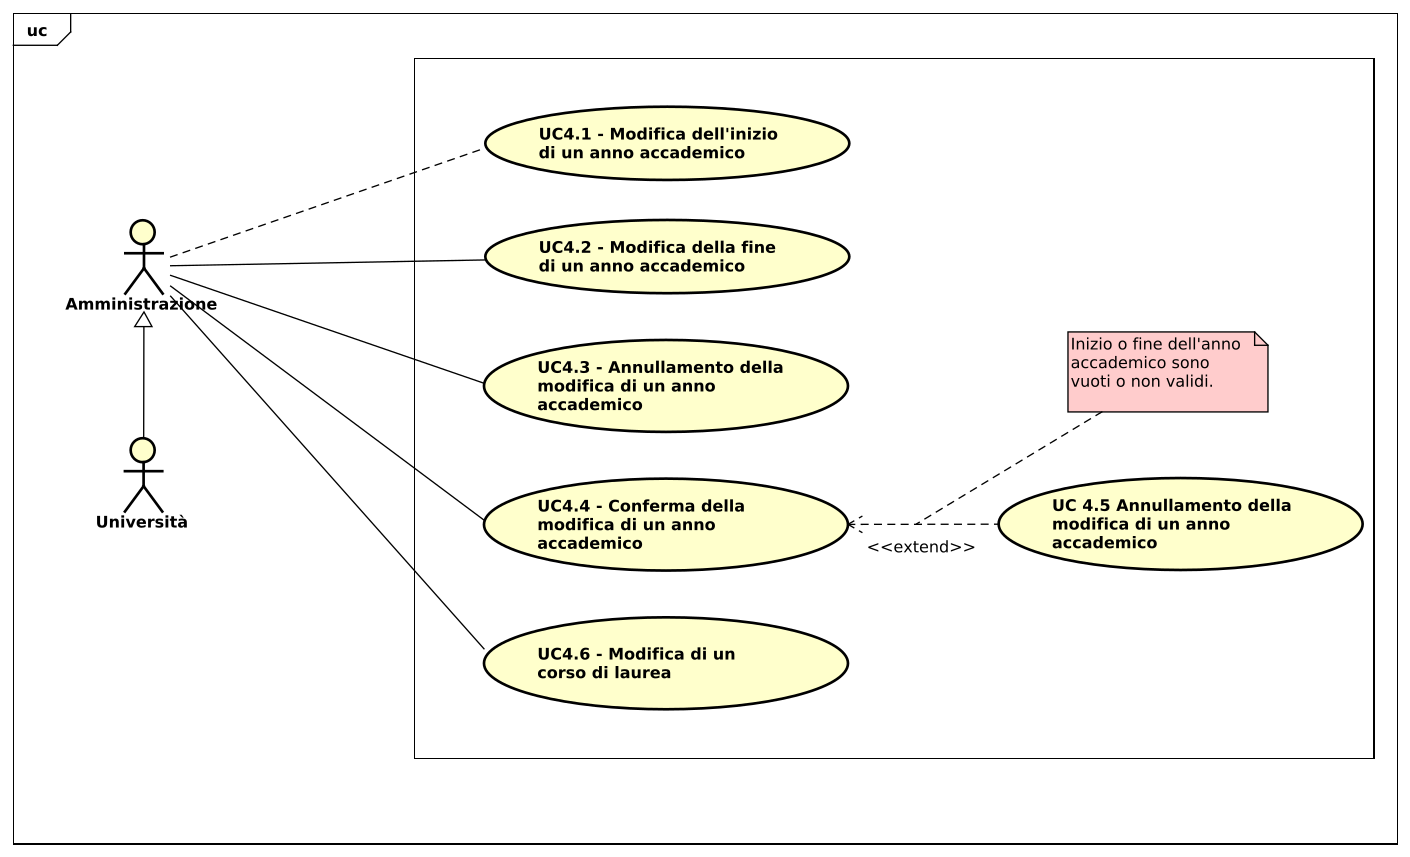
\includegraphics[scale=0.45]{./img/UC4.png}
\caption{Modifica dell'anno accademico}\label{}
\end{figure}
\begin{itemize}
\item \textbf{Attori}: università;
\item \textbf{Descrizione}: L'attore può modificare un anno accademico dalla lista degli anni accademici;
\item \textbf{Precondizione}: La lista degli anni accademici non è vuota e l'attore vuole modificarne uno;
\item \textbf{Flusso principale degli eventi}: L'attore per modificare un anno accademico deve seguire i seguenti punti:
\begin{itemize}
\item Modifica dell'inizio dell'anno accademico (UC4.1)
\item Modifica della fine dell'anno accademico (UC4.2)
\item Annullamento della modifica dell'anno accademico (UC4.3)
\item Conferma della modifica di un anno accademico (UC4.4)
\item Visualizzazione errore relativo alla modifica di un anno accademico (UC4.5)
\end{itemize}
\item \textbf{Postcondizione}: L'attore ha modificato un anno accademico;
\end{itemize}
\subsection{Caso d'uso \texorpdfstring{UC4.1}{UC4.1}: Modifica dell'inizio dell'anno accademico}
\begin{itemize}
\item \textbf{Attori}: università;
\item \textbf{Descrizione}: L'attore modifica la data di partenza dell'anno accademico;
\item \textbf{Precondizione}: L'attore può modificare l'inizio dell'anno accademico;
\item \textbf{Flusso principale degli eventi}: L'attore modifica la data di inizio dell'anno accademico precedentemente inserita;
\item \textbf{Postcondizione}: L'attore ha modificato l'inizio dell'anno accademico;
\end{itemize}
\subsection{Caso d'uso \texorpdfstring{UC4.2}{UC4.2}: Modifica della fine dell'anno accademico}
\begin{itemize}
\item \textbf{Attori}: università;
\item \textbf{Descrizione}: L'attore modifica la data di fine dell'anno accademico;
\item \textbf{Precondizione}: L'attore può modificare la data di fine dell'anno accademico;
\item \textbf{Flusso principale degli eventi}: L'attore modifica la data di fine dell'anno accademico;
\item \textbf{Postcondizione}: L'attore ha modificato la data di fine dell'anno accademico;
\end{itemize}
\subsection{Caso d'uso \texorpdfstring{UC4.3}{UC4.3}: Annullamento della modifica dell'anno accademico}
\begin{itemize}
\item \textbf{Attori}: università;
\item \textbf{Descrizione}: L'attore annulla la modifica dell'anno accademico;
\item \textbf{Precondizione}: L'attore modifica un anno accademico;
\item \textbf{Flusso principale degli eventi}: L'attore una volta iniziata la modifica desidera annullare il processo.
\item \textbf{Postcondizione}: L'attore ha annullato la modifica dell'anno accademico;
\end{itemize}
\subsection{Caso d'uso \texorpdfstring{UC4.4}{UC4.4}: Conferma della modifica di un anno accademico}
\begin{itemize}
\item \textbf{Attori}: università;
\item \textbf{Descrizione}: L'attore conferma la modifica relativa all'anno accademico;
\item \textbf{Precondizione}: L'attore modifica un anno accademico;
\item \textbf{Flusso principale degli eventi}: L'attore ha finito la modifica e desidera inserire nel sistema l'anno accademico modificato.
\item \textbf{Postcondizione}: L'attore ha confermato la modifica di un anno accademico;
\item \textbf{Estensioni}:
\begin{itemize}
\item Visualizzazione errore relativo alla modifica di un anno accademico (UC4.5)
\end{itemize}
\end{itemize}
\subsection{Caso d'uso \texorpdfstring{UC4.5}{UC4.5}: Visualizzazione errore relativo alla modifica di un anno accademico}
\begin{itemize}
\item \textbf{Attori}: università;
\item \textbf{Descrizione}: L'attore può visualizzare un errore nel caso avesse modificato erroneamente dei campi dati;
\item \textbf{Precondizione}: Il sistema ha ricevuto campi dati errati o vuoti;
\item \textbf{Flusso principale degli eventi}: L'attore, modificando in maniera errata i campi dell'anno accademico, può visualizzare uno dei seguenti errori: 
\begin{itemize} \item Inizio dell'anno accademico non valido o lasciato vuoto; \item Fine dell'anno accademico non valido o lasciato vuoto; \item Nome dell'anno accademico non valido o lasciato vuoto. \end{itemize}
\item \textbf{Postcondizione}: Il sistema visualizza un messaggio d'errore;
\end{itemize}
\subsection{Caso d'uso \texorpdfstring{UC5}{UC5}: Eliminazione dell'anno accademico}
\begin{figure} [H]
\centering
\includegraphics[scale=0.45]{./img/UC5.png}
\caption{Eliminazione dell'anno accademico}\label{}
\end{figure}
\begin{itemize}
\item \textbf{Attori}: università;
\item \textbf{Descrizione}: L'attore elimina un anno accademico;
\item \textbf{Precondizione}: L'attore visualizza la lista degli anni accademici e desidera eliminarne uno;
\item \textbf{Flusso principale degli eventi}: L'attore desidera eliminare un anno accademico;
\begin{itemize}
\item Visualizzazione errore relativo all'eliminazione di un anno accademico (UC5.1)
\end{itemize}
\item \textbf{Postcondizione}: L'attore ha eliminato un anno accademico;
\item \textbf{Estensioni}:
\begin{itemize}
\item Visualizzazione errore relativo all'eliminazione di un anno accademico (UC5.1)
\end{itemize}
\end{itemize}
\subsection{Caso d'uso \texorpdfstring{UC5.1}{UC5.1}: Visualizzazione errore relativo all'eliminazione di un anno accademico}
\begin{itemize}
\item \textbf{Attori}: università;
\item \textbf{Descrizione}: Il sistema visualizza un messaggio d'errore riguardante l'impossibilità di eliminazione di un anno accademico.
\item \textbf{Precondizione}: L'attore cerca di eliminare l'anno accademico in corso;
\item \textbf{Flusso principale degli eventi}: L'attore cercando di eliminare l'anno accademico in corso visualizza un messaggio d'errore;
\item \textbf{Postcondizione}: L'attore visualizza un messaggio d'errore riguardante l'impossibilità di eliminare un anno accademico in corso;
\end{itemize}
\subsection{Caso d'uso \texorpdfstring{UC6}{UC6}: Iscrizione ad un esame}
\begin{figure} [H]
\centering
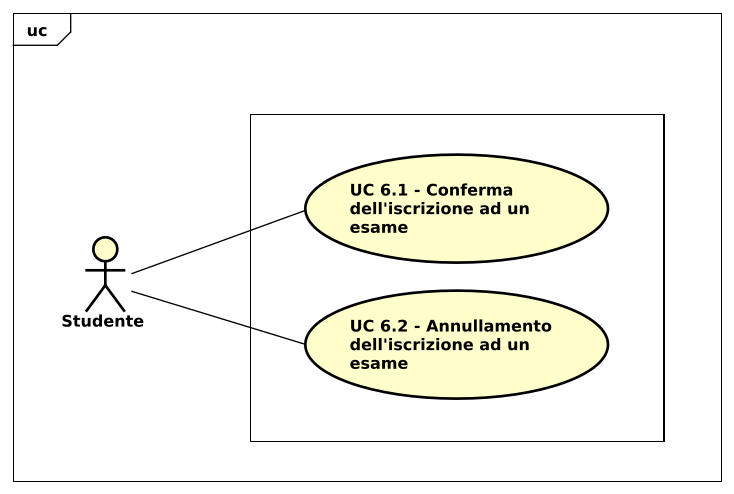
\includegraphics[scale=0.45]{./img/UC6.png}
\caption{Iscrizione ad un esame}\label{}
\end{figure}
\begin{itemize}
\item \textbf{Attori}: studente
\item \textbf{Descrizione}: L'attore vedendo la lista degli appelli disponibili si iscrive ad uno di essi;
\item \textbf{Precondizione}: L'attore vede la lista degli appelli disponibili;
\item \textbf{Flusso principale degli eventi}: L'attore si iscrive ad un esame;
\begin{itemize}
\item Conferma dell'iscrizione ad un esame (UC6.1)
\item Annullamento dell'iscrizione ad un esame (UC6.2)
\end{itemize}
\item \textbf{Postcondizione}: L'attore si è iscritto ad un esame con successo;
\end{itemize}
\subsection{Caso d'uso \texorpdfstring{UC6.1}{UC6.1}: Conferma dell'iscrizione ad un esame}
\begin{itemize}
\item \textbf{Attori}: studente
\item \textbf{Descrizione}: L'attore può confermare l'azione di iscrizione ad un esame.
\item \textbf{Precondizione}: L'attore ha selezionato l'esame a cui si vuole iscrivere;
\item \textbf{Flusso principale degli eventi}: L'attore ha selezionato l'esame a cui iscriversi e può confermare l'azione.
\item \textbf{Postcondizione}: Il sistema ha registrato la scelta dell'attore.
\end{itemize}
\subsection{Caso d'uso \texorpdfstring{UC6.2}{UC6.2}: Annullamento dell'iscrizione ad un esame}
\begin{itemize}
\item \textbf{Attori}: studente
\item \textbf{Descrizione}: L'attore può annullare l'azione di iscrizione ad un esame
\item \textbf{Precondizione}: L'attore ha selezionato l'esame a cui si vuole iscrivere
\item \textbf{Flusso principale degli eventi}: L'attore può annullare l'iscrizione ad un esame dopo averlo selezionato.
\item \textbf{Postcondizione}: L'esame non è più selezionato e l'attore non può confermare l'iscrizione all'esame
\end{itemize}
\subsection{Caso d'uso \texorpdfstring{UC7}{UC7}: Eliminazione dell'iscrizione ad un esame}
\begin{figure} [H]
\centering
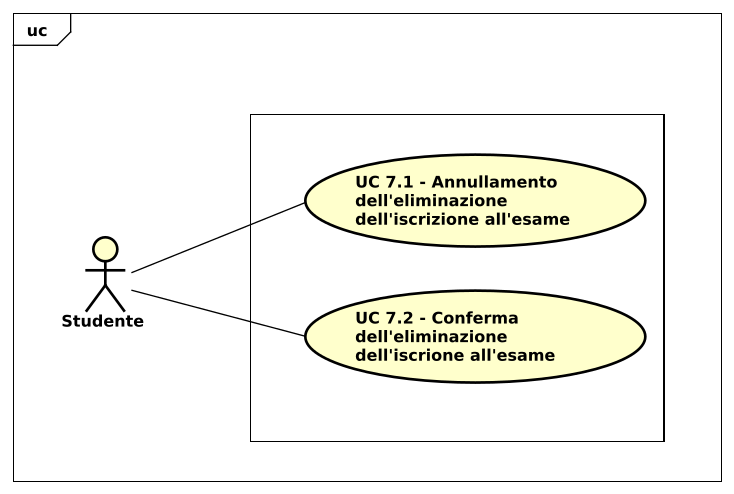
\includegraphics[scale=0.45]{./img/UC7.png}
\caption{Eliminazione dell'iscrizione ad un esame}\label{}
\end{figure}
\begin{itemize}
\item \textbf{Attori}: studente
\item \textbf{Descrizione}: L'attore si è precedentemente iscritto ad un esame e vuole annullarne l'iscrizione;
\item \textbf{Precondizione}: L'attore è registrato ad un esame e vuole eliminare l'iscrizione;
\item \textbf{Flusso principale degli eventi}: L'attore vuole eliminare l'iscrizione ad un esame a cui si è precedentemente registrato;
\begin{itemize}
\item Annullamento dell'eliminazione dell'iscrizione ad un esame (UC7.1)
\item Conferma dell'eliminazione dell'iscrizione ad un esame (UC7.2)
\end{itemize}
\item \textbf{Postcondizione}: L'attore non è più registrato a quell'esame;
\end{itemize}
\subsection{Caso d'uso \texorpdfstring{UC7.1}{UC7.1}: Annullamento dell'eliminazione dell'iscrizione ad un esame}
\begin{itemize}
\item \textbf{Attori}: studente
\item \textbf{Descrizione}: L'attore sta eliminando l'iscrizione ad un esame ma decide di non farlo
\item \textbf{Precondizione}: L'attore sta eliminando l'iscrizione ad un esame;
\item \textbf{Flusso principale degli eventi}: L'attore che sta eliminando l'iscrizione ad un esame decide di annullare l'operazione;
\item \textbf{Postcondizione}: L'attore non ha eliminato l'iscrizione a quell'esame;
\end{itemize}
\subsection{Caso d'uso \texorpdfstring{UC7.2}{UC7.2}: Conferma dell'eliminazione dell'iscrizione ad un esame}
\begin{itemize}
\item \textbf{Attori}: professore
\item \textbf{Descrizione}: L'attore che sta eliminando l'iscrizione ad un esame, conferma tale scelta;
\item \textbf{Precondizione}: L'attore sta eliminando l'iscrizione ad un esame;
\item \textbf{Flusso principale degli eventi}: L'attore conferma l'eliminazione di un'iscrizione ad un esame;
\item \textbf{Postcondizione}: L'attore ha eliminato l'iscrizione ad un esame;
\end{itemize}
\subsection{Caso d'uso \texorpdfstring{UC8}{UC8}: Rifiuto del voto di un esame}
\begin{itemize}
\item \textbf{Attori}: studente
\item \textbf{Descrizione}: L'attore può rifiutare il voto di un esame;
\item \textbf{Precondizione}: L'attore visualizza il voto di un esame;
\item \textbf{Flusso principale degli eventi}: L'attore dopo aver visualizzato il voto dell'esame decide di rifiutarne il voto;
\item \textbf{Postcondizione}: L'attore rifiuta il voto dell'esame;
\end{itemize}
\subsection{Caso d'uso \texorpdfstring{UC9}{UC9}: Modifica dell'esame da parte di un professore}
\begin{figure} [H]
\centering
\includegraphics[scale=0.45]{./img/UC9.png}
\caption{Modifica dell'esame da parte di un professore}\label{}
\end{figure}
\begin{itemize}
\item \textbf{Attori}: professore
\item \textbf{Descrizione}: L'attore ha accesso alla modifica di alcuni campi dati degli esami a cui sono assegnati.
\item \textbf{Precondizione}: L'attore può modificare parzialmente un esame;
\item \textbf{Flusso principale degli eventi}: L'attore ha possibilità di modifica dei seguenti punti degli esami a cui è assegnato:
\begin{itemize}
\item Modifica dell'intervallo di prenotazione di un esame (UC9.1)
\item Modifica della data di un esame (UC9.2)
\item Modifica del luogo di un esame (UC9.3)
\item Annullamento modifica esame (UC9.4)
\item Conferma modifiche di un esame (UC9.5)
\item Visualizzazione errore di modifica esame (UC9.6)
\end{itemize}
\item \textbf{Postcondizione}: L'attore ha modificato l'esame;
\end{itemize}
\subsection{Caso d'uso \texorpdfstring{UC9.1}{UC9.1}: Modifica dell'intervallo di prenotazione di un esame}
\begin{itemize}
\item \textbf{Attori}: professore
\item \textbf{Descrizione}: L'attore modifica l'intervallo temporale per cui uno studente ha la possibilità di iscriversi ad un esame;
\item \textbf{Precondizione}: Il sistema visualizza l'opzione di modifica dell'intervallo di prenotazione di un esame;
\item \textbf{Flusso principale degli eventi}: L'attore modifica l'intervallo di prenotazione di un esame;
\item \textbf{Postcondizione}: L'attore ha modificato l'intervallo di prenotazione di un esame;
\end{itemize}
\subsection{Caso d'uso \texorpdfstring{UC9.2}{UC9.2}: Modifica della data di un esame}
\begin{itemize}
\item \textbf{Attori}: professore
\item \textbf{Descrizione}: L'attore ha la possibilità di modificare la data di un esame;
\item \textbf{Precondizione}: L'attore sta modificando un esame;
\item \textbf{Flusso principale degli eventi}: L'attore modifica la data di un esame.
\item \textbf{Postcondizione}: L'attore ha modificato l'ora di un esame;
\end{itemize}
\subsection{Caso d'uso \texorpdfstring{UC9.3}{UC9.3}: Modifica del luogo di un esame}
\begin{itemize}
\item \textbf{Attori}: professore
\item \textbf{Descrizione}: L'attore ha la possibilità di modificare il luogo degli esami a cui è assegnato;
\item \textbf{Precondizione}: L'attore sta modificando un esame;
\item \textbf{Flusso principale degli eventi}: L'attore modifica il luogo di un esame;
\item \textbf{Postcondizione}: L'attore ha modificato il luogo di un esame;
\end{itemize}
\subsection{Caso d'uso \texorpdfstring{UC9.4}{UC9.4}: Annullamento modifica esame}
\begin{itemize}
\item \textbf{Attori}: professore
\item \textbf{Descrizione}: L'attore che sta modificando un esame, decide di annullare l'operazione;
\item \textbf{Precondizione}: L'attore sta modificando un esame;
\item \textbf{Flusso principale degli eventi}: L'attore annulla le modifiche che sta compiendo.
\item \textbf{Postcondizione}: L'attore ha annullato le modifiche all'esame;
\end{itemize}
\subsection{Caso d'uso \texorpdfstring{UC9.5}{UC9.5}: Conferma modifiche di un esame}
\begin{itemize}
\item \textbf{Attori}: professore
\item \textbf{Descrizione}: L'attore che sta modificando un esame decide di confermare le modifiche;
\item \textbf{Precondizione}: L'attore sta modificando un esame;
\item \textbf{Flusso principale degli eventi}: L'attore conferma le modifiche fatte all'esame;
\item \textbf{Postcondizione}: L'attore ha confermato le modifiche relative all'esame;
\item \textbf{Estensioni}:
\begin{itemize}
\item Visualizzazione errore di modifica esame (UC9.6)
\end{itemize}
\end{itemize}
\subsection{Caso d'uso \texorpdfstring{UC9.6}{UC9.6}: Visualizzazione errore di modifica esame}
\begin{itemize}
\item \textbf{Attori}: professore
\item \textbf{Descrizione}: Il sistema visualizza un errore riguardante l'errata modifica dei campi dati di un esame;
\item \textbf{Precondizione}: L'attore sta modificando un esame;
\item \textbf{Flusso principale degli eventi}: L'attore, modificando in maniera errata i campi dell'esame, può visualizzare uno dei seguenti errori: \begin{itemize}
\item Intervallo di prenotazione per l’esame non valido o lasciato vuoto;
\item Data dell’esame non valida o lasciato vuoto;
\item Luogo d’esame non valido o lasciato vuoto;
\end{itemize}
\item \textbf{Postcondizione}: L'attore visualizza un messaggio d'errore riguardante l'errata modifica dell'esame.
\end{itemize}
\subsection{Caso d'uso \texorpdfstring{UC10}{UC10}: Inserimento voto }
\begin{figure} [H]
\centering
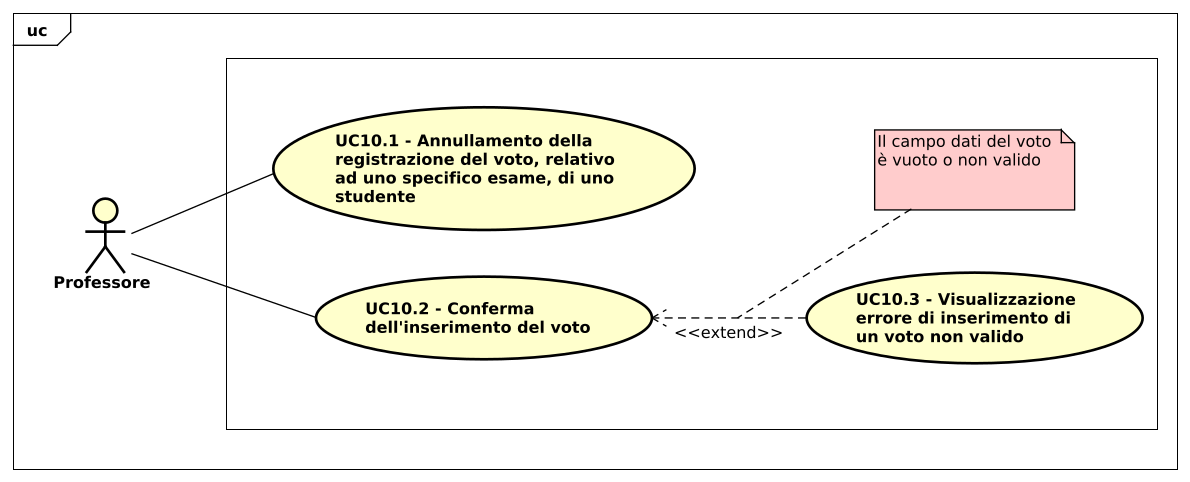
\includegraphics[scale=0.45]{./img/UC10.png}
\caption{Inserimento voto }\label{}
\end{figure}
\begin{itemize}
\item \textbf{Attori}: professore
\item \textbf{Descrizione}: L'attore visualizza la lista degli studenti iscritti all'esame e assegna una votazione;
\item \textbf{Precondizione}: L'attore visualizza la lista degli studenti iscritti all'esame;
\item \textbf{Flusso principale degli eventi}: L'attore inserisce un voto ad uno studente;
\begin{itemize}
\item Annullamento della registrazione del voto, relativo ad uno specifico esame, di uno studente (UC10.1)
\item Conferma dell'inserimento del voto (UC10.2)
\item Visualizzazione errore di inserimento di un voto non valido (UC10.3)
\end{itemize}
\item \textbf{Postcondizione}: L'attore inserisce il voto allo studente;
\end{itemize}
\subsection{Caso d'uso \texorpdfstring{UC10.1}{UC10.1}: Annullamento della registrazione del voto, relativo ad uno specifico esame, di uno studente}
\begin{itemize}
\item \textbf{Attori}: professore
\item \textbf{Descrizione}: L'attore sta inserendo il voto ad uno studente e decide di annullare l'operazione;
\item \textbf{Precondizione}: L'attore sta inserendo il voto ad uno studente;
\item \textbf{Flusso principale degli eventi}: L'attore che sta inserendo un voto può decidere di annullare l'operazione;
\item \textbf{Postcondizione}: L'attore ha annullato l'operazione di inserimento del voto;
\end{itemize}
\subsection{Caso d'uso \texorpdfstring{UC10.2}{UC10.2}: Conferma dell'inserimento del voto}
\begin{itemize}
\item \textbf{Attori}: professore
\item \textbf{Descrizione}: L'attore dopo aver immesso il voto dello studete decide di confermarlo;
\item \textbf{Precondizione}: L'attore sta inserendo il voto allo studente;
\item \textbf{Flusso principale degli eventi}: L'attore che inserisce il voto allo studente può confermarlo;
\item \textbf{Postcondizione}: L'attore ha ha confermato l'inserimento del voto;
\item \textbf{Estensioni}:
\begin{itemize}
\item Visualizzazione errore di inserimento di un voto non valido (UC10.3)
\end{itemize}
\end{itemize}
\subsection{Caso d'uso \texorpdfstring{UC10.3}{UC10.3}: Visualizzazione errore di inserimento di un voto non valido}
\begin{itemize}
\item \textbf{Attori}: professore
\item \textbf{Descrizione}: Il sistema visualizza un messaggio di errore causato dall'immissione di un voto non conforme;
\item \textbf{Precondizione}: L'attore inserisce il voto;
\item \textbf{Flusso principale degli eventi}: L'attore, che sbaglia ad inserire un voto, visualizza un messaggio d'errore relativo ad esso,
\item \textbf{Postcondizione}: L'attore visualizza un messaggio d'errore relativo all'aggiunta errata del voto;
\end{itemize}
\subsection{Caso d'uso \texorpdfstring{UC11}{UC11}: Inserimento dell'utente nel sistema}
\begin{figure} [H]
\centering
\includegraphics[scale=0.45]{./img/UC11.png}
\caption{Inserimento dell'utente nel sistema}\label{}
\end{figure}
\begin{itemize}
\item \textbf{Attori}: università;
\item \textbf{Descrizione}: L'attore può inserire un nuovo utente nel sistema
\item \textbf{Precondizione}: L'utente da inserire non è presente nel sistema
\item \textbf{Flusso principale degli eventi}: L'attore può inserire un nuovo utente nel sistema e questo non è già presente
\begin{itemize}
\item Inserimento della matricola relativa all'utente (UC11.1)
\item Inserimento del codice univoco relativo all'utente (UC11.2)
\item Inserimento della tipologia dell'utente (UC11.3)
\item Conferma dell'inserimento dell'utente nel sistema (UC11.4)
\item Visualizzazione errore relativo all'inserimento di un utente nel sistema (UC11.5)
\item Annullamento dell'inserimento di un nuovo utente nel sistema (UC11.6)
\end{itemize}
\item \textbf{Postcondizione}: L'utente è presente nel sistema
\end{itemize}
\subsection{Caso d'uso \texorpdfstring{UC11.1}{UC11.1}: Inserimento della matricola relativa all'utente}
\begin{itemize}
\item \textbf{Attori}: università;
\item \textbf{Descrizione}: L'attore può inserire la matricola relativa all'utente
\item \textbf{Precondizione}: L'attore non ha ancora inserito la matricola relativa all'utente
\item \textbf{Flusso principale degli eventi}: L'attore può inserire la matricola dell'utente durante il suo inserimento nel sistema
\item \textbf{Postcondizione}: L'attore può aver inserito la matricola relativa all'utente
\end{itemize}
\subsection{Caso d'uso \texorpdfstring{UC11.2}{UC11.2}: Inserimento del codice univoco relativo all'utente}
\begin{itemize}
\item \textbf{Attori}: università;
\item \textbf{Descrizione}: L'attore può inserire il codice univoco relativo all'utente
\item \textbf{Precondizione}: L'attore non ha ancora inserito il codice univoco relativo all'utente
\item \textbf{Flusso principale degli eventi}: L'attore può inserire il codice univoco dell'utente durante il suo inserimento nel sistema
\item \textbf{Postcondizione}: L'attore può aver inserito il codice univoco relativo all'utente
\end{itemize}
\subsection{Caso d'uso \texorpdfstring{UC11.3}{UC11.3}: Inserimento della tipologia dell'utente}
\begin{itemize}
\item \textbf{Attori}: università;
\item \textbf{Descrizione}: L'attore può inserire la tipologia relativa all'utente
\item \textbf{Precondizione}: L'attore non ha ancora inserito la tipologia relativa all'utente
\item \textbf{Flusso principale degli eventi}: L'attore può inserire la tipologia dell'utente durante il suo inserimento nel sistema. Potrà scegliere tra:
\begin{itemize}
\item Professore
\item Studente
\end{itemize}
\item \textbf{Postcondizione}: L'attore può aver inserito la tipologia relativa all'utente
\end{itemize}
\subsection{Caso d'uso \texorpdfstring{UC11.4}{UC11.4}: Conferma dell'inserimento dell'utente nel sistema}
\begin{itemize}
\item \textbf{Attori}: università;
\item \textbf{Descrizione}: L'attore può confermare l'inserimento nel sistema.
\item \textbf{Precondizione}: L'utente da inserire non è ancora presente nel sistema.
\item \textbf{Flusso principale degli eventi}: L'attore può confermare l'inserimento dell'utente nel sistema
\item \textbf{Postcondizione}: L'utente è stato inserito nel sistema con successo.
\item \textbf{Estensioni}:
\begin{itemize}
\item Visualizzazione errore relativo all'inserimento di un utente nel sistema (UC11.5)
\end{itemize}
\end{itemize}
\subsection{Caso d'uso \texorpdfstring{UC11.5}{UC11.5}: Visualizzazione errore relativo all'inserimento di un utente nel sistema}
\begin{itemize}
\item \textbf{Attori}: università;
\item \textbf{Descrizione}: L'attore aggiunge i dettagli relativi all'inserimento di un utente nel sistema senza rispettarne la validazione.
\item \textbf{Precondizione}: L'attore inserisce i campi dati dell'utente
\item \textbf{Flusso principale degli eventi}: L'attore, impostando in maniera errata i campi dell'utente, può visualizzare uno dei seguenti errori:
\begin{itemize}
\item Matricola non valida oppure lasciata vuota;
\item Codice univoco non valido oppure lasciato vuoto
\end{itemize}
\item \textbf{Postcondizione}: L'attore visualizza un messaggio d'errore riguardante l'aggiunta errata di uno o più campi dati dell'utente
\end{itemize}
\subsection{Caso d'uso \texorpdfstring{UC11.6}{UC11.6}: Annullamento dell'inserimento di un nuovo utente nel sistema}
\begin{itemize}
\item \textbf{Attori}: università;
\item \textbf{Descrizione}: L'attore non inserisce più un nuovo utente nel sistema
\item \textbf{Precondizione}: L'attore può aver inserito dei campi dati relativi ad un utente
\item \textbf{Flusso principale degli eventi}: L'attore non inserisce più un nuovo utente nel sistema e quindi annulla l'operazione
\item \textbf{Postcondizione}: L'attore non può più inserire altri campi dati relativi all'inserimento di un nuovo utente nel sistema
\end{itemize}
\subsection{Caso d'uso \texorpdfstring{UC12}{UC12}: Rimozione dell'utente dal sistema}
\begin{figure} [H]
\centering
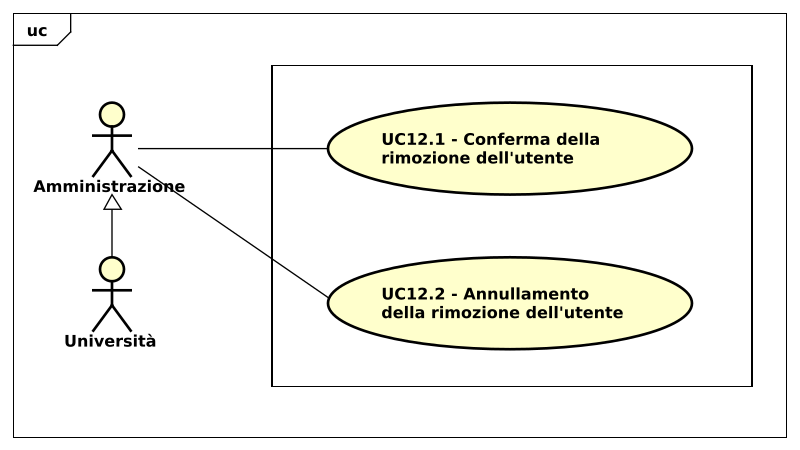
\includegraphics[scale=0.45]{./img/UC12.png}
\caption{Rimozione dell'utente dal sistema}\label{}
\end{figure}
\begin{itemize}
\item \textbf{Attori}: università;
\item \textbf{Descrizione}: L'attore può rimuovere un utente, cancellandone tutti i dati ad esso associati nonché rimuovendone l'accesso al sistema
\item \textbf{Precondizione}: L'utente è registrato all'interno del sistema
\item \textbf{Flusso principale degli eventi}: L'attore può rimuovere completamente un utente dal sistema
\begin{itemize}
\item Conferma della rimozione di un utente dal sistema (UC12.1)
\item Annullamento della rimozione di un utente dal sistema (UC12.2)
\end{itemize}
\item \textbf{Postcondizione}: L'utente non è più registrato nel sistema e tutti i suoi dati sono stati cancellati;
\end{itemize}
\subsection{Caso d'uso \texorpdfstring{UC12.1}{UC12.1}: Conferma della rimozione di un utente dal sistema}
\begin{itemize}
\item \textbf{Attori}: università;
\item \textbf{Descrizione}: L'attore può confermare la rimozione di un utente dal sistema
\item \textbf{Precondizione}: L'attore ha selezionato l'utente da rimuovere dal sistema
\item \textbf{Flusso principale degli eventi}: L'attore può confermare la rimozione di un utente dal sistema
\item \textbf{Postcondizione}: L'utente è effettivamente rimosso dal sistema
\end{itemize}
\subsection{Caso d'uso \texorpdfstring{UC12.2}{UC12.2}: Annullamento della rimozione di un utente dal sistema}
\begin{itemize}
\item \textbf{Attori}: università;
\item \textbf{Descrizione}: L'attore può annullare la rimozione di un utente dal sistema
\item \textbf{Precondizione}: L'attore ha selezionato l'utente da rimuovere dal sistema
\item \textbf{Flusso principale degli eventi}: L'attore può annullare l'azione di rimozione di un utente dal sistema
\item \textbf{Postcondizione}: L'attore ha annullato la selezione dell'utente da rimuovere dal sistema
\end{itemize}
